\chapter{\protect\hyperlink{:}{力学}}
\addtocontents{toc}{\protect\hypertarget{:}{}}


\section{\protect\hyperlink{:}{质点运动学}}
\addtocontents{toc}{\protect\hypertarget{:}{}}

\subsection{\protect\hyperlink{:}{为什么要研究运动学？}}
\addtocontents{toc}{\protect\hypertarget{:}{}}

在学习力学之前，我们首先需要回答一个最基本的问题：\textbf{如何描述一个物体的运动？}

这个问题看似简单，实则蕴含着深刻的思考。试想一下，一个球在空中飞行——我们需要用什么样的数学语言来精确地描述它的运动状态？显然，仅仅说"球在动"是远远不够的。我们需要知道：
\begin{enumerate}
    \item 球在某一时刻处于什么\textbf{位置}？
    \item 球的\textbf{位置}如何随时间\textbf{变化}？（即速度）
    \item 球的\textbf{速度}如何随时间\textbf{变化}？（即加速度）
\end{enumerate}

运动学的任务，就是建立一套数学框架来回答这些问题。注意，运动学只关心"如何描述运动"，而关心"为什么物体会这样运动"——后者是动力学的内容。

\subsection{\protect\hyperlink{:}{质点模型}}
\addtocontents{toc}{\protect\hypertarget{:}{}}

现实中的物体都有大小和形状，直接描述其运动非常复杂。为了简化问题，我们引入第一个理想化模型——\textbf{质点}。

\begin{definition}[质点]
    当物体的大小和形状对所研究的问题没有影响，或者影响可以忽略不计时，我们可以将物体抽象为一个具有质量但没有大小的点，称为\textbf{质点}。
\end{definition}

一个物体能否被看作质点，取决于所研究的具体问题。例如：
\begin{enumerate}
    \item 研究地球绕太阳的公转时，地球的直径（约 $1.3 \times 10^4$ km）远小于日地距离（约 $1.5 \times 10^8$ km），可以将地球看作质点。
    \item 研究地球的自转时，地球上不同位置的运动状态不同，不能将其看作质点。
\end{enumerate}

\subsection{\protect\hyperlink{:}{直角坐标系中的运动描述}}
\addtocontents{toc}{\protect\hypertarget{:}{}}

有了质点模型，接下来我们需要选择一个\textbf{参考系}来描述运动。参考系的选择是任意的，但选择合适的参考系可以大大简化问题。

最自然的选择是\textbf{直角坐标系}（也称笛卡尔坐标系）。在直角坐标系中，我们用一组固定的基矢 $\hat{i}$、$\hat{j}$（二维情况）来描述空间中的方向，它们的大小和方向都不随时间变化——这是一个巨大的优势。

\subsubsection{\protect\hyperlink{:}{位矢、位移}}
\addtocontents{toc}{\protect\hypertarget{:}{}}

要描述质点的位置，我们引入\textbf{位矢}（位置矢量）的概念：

\begin{definition}[位矢]
    位矢是从坐标原点指向质点所在位置的矢量，记作 $\vec{r}$。在二维直角坐标系中
    \begin{equation}
        \vec{r} = x\hat{i} + y\hat{j}
    \end{equation}
    其中 $x$、$y$ 分别是质点在两个坐标轴上的坐标。
\end{definition}

\begin{figure}[htbp]
    \centering
    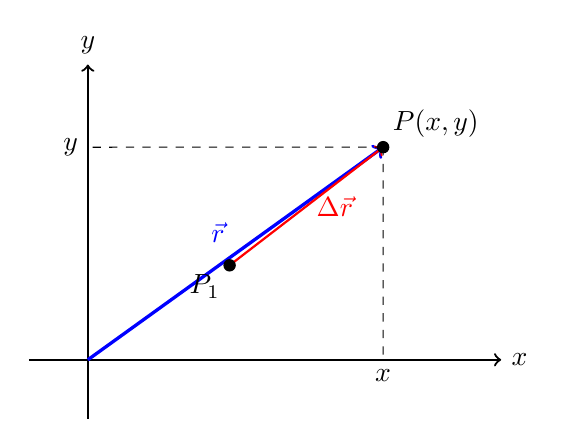
\begin{tikzpicture}[scale=1.5]
        \draw[->,thick] (-0.5,0) -- (3.5,0) node[right]{$x$};
        \draw[->,thick] (0,-0.5) -- (0,2.5) node[above]{$y$};
        \coordinate (O) at (0,0);
        \coordinate (P) at (2.5,1.8);
        \coordinate (P1) at (1.2,0.8);
        \coordinate (P2) at (2.5,1.8);
        \draw[->,very thick,blue] (O) -- (P) node[midway,above left]{$\vec{r}$};
        \draw[->,thick,red] (P1) -- (P2) node[midway,right]{$\Delta\vec{r}$};
        \fill (P) circle (1.5pt) node[above right]{$P(x,y)$};
        \fill (P1) circle (1.5pt) node[below left]{$P_1$};
        \draw[dashed] (P) -- (2.5,0) node[below]{$x$};
        \draw[dashed] (P) -- (0,1.8) node[left]{$y$};
    \end{tikzpicture}
    \caption{位矢与位移}
    \label{fig:位矢与位移}
\end{figure}

当质点从位置 $P_1$ 运动到 $P_2$ 时，其位置的变化用\textbf{位移}矢量描述
\begin{equation}
    \Delta\vec{r} = \vec{r}_2 - \vec{r}_1 = (x_2 - x_1)\hat{i} + (y_2 - y_1)\hat{j}
\end{equation}

注意区分\textbf{位移}和\textbf{路程}：位移是矢量，只与始末位置有关；路程是标量，是质点实际走过的路径长度。

\subsubsection{\protect\hyperlink{:}{速度}}
\addtocontents{toc}{\protect\hypertarget{:}{}}

位移告诉我们质点"去了哪里"，但没有告诉我们"去得有多快"。为了描述运动的快慢，我们引入\textbf{速度}。

直觉上，速度是"单位时间内的位移"。但如果时间间隔不是无穷小，这个比值只是\textbf{平均速度}。要得到质点在某一时刻的真实运动状态，我们需要取极限——这就是\textbf{瞬时速度}。

\begin{definition}[瞬时速度]
    瞬时速度是位矢对时间的导数
    \begin{equation}
        \vec{v} = \frac{\mathrm{d}\vec{r}}{\mathrm{d}t} = \lim_{\Delta t \to 0} \frac{\Delta\vec{r}}{\Delta t}
    \end{equation}
\end{definition}

在直角坐标系中，由于基矢不随时间变化，求导可以分量进行
\begin{equation}
    \vec{v} = \frac{\mathrm{d}\vec{r}}{\mathrm{d}t} = \frac{\mathrm{d}x}{\mathrm{d}t}\hat{i} + \frac{\mathrm{d}y}{\mathrm{d}t}\hat{j} = v_x\hat{i} + v_y\hat{j}
\end{equation}

速度的大小（速率）为
\begin{equation}
    v = |\vec{v}| = \sqrt{v_x^2 + v_y^2}
\end{equation}

速度的方向沿质点运动轨迹的切线方向——这是瞬时速度的一个重要几何特征。

\subsubsection{\protect\hyperlink{:}{加速度}}
\addtocontents{toc}{\protect\hypertarget{:}{}}

同样地，速度也可能随时间变化。描述速度变化快慢的物理量是\textbf{加速度}。

\begin{definition}[瞬时加速度]
    瞬时加速度是速度对时间的导数，即位矢对时间的二阶导数
    \begin{equation}
        \vec{a} = \frac{\mathrm{d}\vec{v}}{\mathrm{d}t} = \frac{\mathrm{d}^2\vec{r}}{\mathrm{d}t^2}
    \end{equation}
\end{definition}

在直角坐标系中
\begin{equation}
    \vec{a} = \frac{\mathrm{d}v_x}{\mathrm{d}t}\hat{i} + \frac{\mathrm{d}v_y}{\mathrm{d}t}\hat{j} = a_x\hat{i} + a_y\hat{j}
\end{equation}

\begin{remark}
    加速度的方向与速度的方向一般不同。加速度描述的是速度\textbf{大小和方向}的变化率，而不仅仅是速率的变化。即使速率不变（匀速圆周运动），只要速度方向在改变，加速度就不为零。
\end{remark}

总结一下，在直角坐标系中，运动学量的描述非常简洁
\begin{equation}
    \boxed{
        \vec{r} = x\hat{i} + y\hat{j}, \quad
        \vec{v} = \dot{x}\hat{i} + \dot{y}\hat{j}, \quad
        \vec{a} = \ddot{x}\hat{i} + \ddot{y}\hat{j}
    }
\end{equation}

其中上方的点表示对时间求导。这种简洁性正是直角坐标系的优势所在——基矢不随时间变化，求导可以完全分量独立地进行。

\subsection{\protect\hyperlink{:}{极坐标系中的运动描述}}
\addtocontents{toc}{\protect\hypertarget{:}{}}

直角坐标系虽然简洁，但并非总是最佳选择。考虑一个简单的例子：一个质点绕某一点做圆周运动。在直角坐标系中，质点的坐标为
\begin{equation}
    x = R\cos\omega t, \qquad y = R\sin\omega t
\end{equation}

虽然可以描述，但每次都要处理三角函数，很不方便。如果改用极坐标 $(r, \theta)$，问题就变得简单了——圆周运动只需要 $r = R$、$\theta = \omega t$，非常简洁。

更一般地，对于那些具有某种对称性的运动（如行星绕太阳的运动），极坐标系往往是更自然的选择。

\subsubsection{\protect\hyperlink{:}{极坐标系的基矢}}
\addtocontents{toc}{\protect\hypertarget{:}{}}

在极坐标系中，我们用 $(r, \theta)$ 来描述质点的位置，其中 $r$ 是到原点的距离，$\theta$ 是与极轴（通常取 $x$ 轴）的夹角。

位矢表示为
\begin{equation}
    \vec{r} = r\hat{e}_r
\end{equation}

其中 $\hat{e}_r$ 是沿径向的单位矢量，$\hat{e}_\theta$ 是沿横向（垂直于 $\hat{e}_r$，指向 $\theta$ 增大的方向）的单位矢量。

\begin{figure}[htbp]
    \centering
    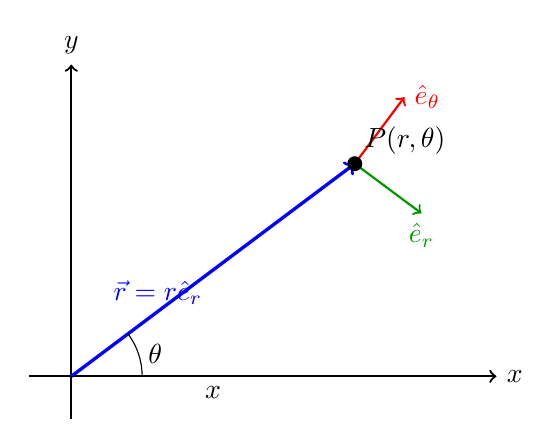
\begin{tikzpicture}[scale=1.8]
        \draw[->,thick] (-0.3,0) -- (3,0) node[right]{$x$};
        \draw[->,thick] (0,-0.3) -- (0,2.2) node[above]{$y$};
        \coordinate (O) at (0,0);
        \coordinate (P) at (2,1.5);
        \draw[->,very thick,blue] (O) -- (P) node[midway,below left]{$\vec{r} = r\hat{e}_r$};
        \draw[->,thick,red] (P) -- ++(0.35,0.47) node[right]{$\hat{e}_\theta$};
        \draw[->,thick,green!60!black] (P) -- ++(0.47,-0.35) node[below]{$\hat{e}_r$};
        \draw[dashed] (O) -- (2,0) node[midway,below]{$x$};
        \draw (0.5,0) arc (0:36.87:0.5) node[midway,right]{$\theta$};
        \fill (P) circle (1.5pt) node[above right]{$P(r,\theta)$};
    \end{tikzpicture}
    \caption{极坐标系中的基矢}
    \label{fig:极坐标系基矢}
\end{figure}

与直角坐标系不同，极坐标系的基矢 $\hat{e}_r$ 和 $\hat{e}_\theta$ 的方向随 $\theta$ 变化——这是极坐标系的核心特点，也是推导速度和加速度公式时必须特别注意的地方。

\subsubsection{\protect\hyperlink{:}{基矢的导数}}
\addtocontents{toc}{\protect\hypertarget{:}{}}

由于基矢的方向在变化，当我们对位矢求导时，不仅要考虑 $r$ 的变化，还要考虑 $\hat{e}_r$ 的变化。因此，我们需要先搞清楚基矢对时间的导数是什么。

将极坐标基矢用直角坐标基矢表示
\begin{align}
    \hat{e}_r &= \cos\theta\,\hat{i} + \sin\theta\,\hat{j} \\
    \hat{e}_\theta &= -\sin\theta\,\hat{i} + \cos\theta\,\hat{j}
\end{align}

对时间求导（注意 $\hat{i}$、$\hat{j}$ 是常矢量，只有 $\theta$ 是时间的函数），利用链式法则 $\dfrac{\mathrm{d}}{\mathrm{d}t} = \dfrac{\mathrm{d}}{\mathrm{d}\theta}\dfrac{\mathrm{d}\theta}{\mathrm{d}t}$
\begin{align}
    \frac{\mathrm{d}\hat{e}_r}{\mathrm{d}t} &= (-\sin\theta\,\hat{i} + \cos\theta\,\hat{j})\dot{\theta} = \dot{\theta}\,\hat{e}_\theta \\
    \frac{\mathrm{d}\hat{e}_\theta}{\mathrm{d}t} &= (-\cos\theta\,\hat{i} - \sin\theta\,\hat{j})\dot{\theta} = -\dot{\theta}\,\hat{e}_r
\end{align}

这两个关系非常重要，可以总结为
\begin{equation}
    \boxed{
        \frac{\mathrm{d}\hat{e}_r}{\mathrm{d}t} = \dot{\theta}\hat{e}_\theta, \qquad
        \frac{\mathrm{d}\hat{e}_\theta}{\mathrm{d}t} = -\dot{\theta}\hat{e}_r
    }
\end{equation}

\begin{remark}
    直觉上，当 $\theta$ 增大时，$\hat{e}_r$ 向 $\hat{e}_\theta$ 方向旋转，所以 $\dot{\hat{e}_r}$ 沿 $\hat{e}_\theta$ 方向；同理，$\hat{e}_\theta$ 向 $-\hat{e}_r$ 方向旋转，所以 $\dot{\hat{e}_\theta}$ 沿 $-\hat{e}_r$ 方向。大小都是 $\dot{\theta}$，因为单位矢量的长度不变，只改变方向。
\end{remark}

\subsubsection{\protect\hyperlink{:}{极坐标系中的速度}}
\addtocontents{toc}{\protect\hypertarget{:}{}}

有了基矢的导数，我们就可以推导极坐标系中的速度公式了。从 $\vec{r} = r\hat{e}_r$ 出发
\begin{equation}
    \vec{v} = \frac{\mathrm{d}\vec{r}}{\mathrm{d}t} = \frac{\mathrm{d}r}{\mathrm{d}t}\hat{e}_r + r\frac{\mathrm{d}\hat{e}_r}{\mathrm{d}t} = \dot{r}\hat{e}_r + r\dot{\theta}\hat{e}_\theta
\end{equation}

\begin{equation}
    \boxed{
        \vec{v} = \underbrace{\dot{r}\hat{e}_r}_{\text{径向速度}} + \underbrace{r\dot{\theta}\hat{e}_\theta}_{\text{横向速度}}
    }
\end{equation}

速度有两个分量：
\begin{enumerate}
    \item \textbf{径向速度} $v_r = \dot{r}$：沿 $\hat{e}_r$ 方向，描述质点远离或靠近原点的快慢。
    \item \textbf{横向速度} $v_\theta = r\dot{\theta}$：沿 $\hat{e}_\theta$ 方向，描述质点绕原点转动的快慢。
\end{enumerate}

\begin{remark}
    对于圆周运动（$r = R = \text{常量}$），$\dot{r} = 0$，所以 $v = R\dot{\theta} = R\omega$，与我们熟悉的公式一致。
\end{remark}

\subsubsection{\protect\hyperlink{:}{极坐标系中的加速度}}
\addtocontents{toc}{\protect\hypertarget{:}{}}

对速度再求一次时间导数
\begin{align}
    \vec{a} &= \frac{\mathrm{d}\vec{v}}{\mathrm{d}t} = \frac{\mathrm{d}}{\mathrm{d}t}\left(\dot{r}\hat{e}_r + r\dot{\theta}\hat{e}_\theta\right) \nonumber \\
    &= \ddot{r}\hat{e}_r + \dot{r}\frac{\mathrm{d}\hat{e}_r}{\mathrm{d}t} + \dot{r}\dot{\theta}\hat{e}_\theta + r\ddot{\theta}\hat{e}_\theta + r\dot{\theta}\frac{\mathrm{d}\hat{e}_\theta}{\mathrm{d}t} \nonumber \\
    &= \ddot{r}\hat{e}_r + \dot{r}\dot{\theta}\hat{e}_\theta + \dot{r}\dot{\theta}\hat{e}_\theta + r\ddot{\theta}\hat{e}_\theta - r\dot{\theta}^2\hat{e}_r \nonumber \\
    &= (\ddot{r} - r\dot{\theta}^2)\hat{e}_r + (r\ddot{\theta} + 2\dot{r}\dot{\theta})\hat{e}_\theta
\end{align}

\begin{equation}
    \boxed{
        \vec{a} = \underbrace{(\ddot{r} - r\dot{\theta}^2)}_{a_r}\hat{e}_r + \underbrace{(r\ddot{\theta} + 2\dot{r}\dot{\theta})}_{a_\theta}\hat{e}_\theta
    }
\end{equation}

加速度也有两个分量：
\begin{enumerate}
    \item \textbf{径向加速度} $a_r = \ddot{r} - r\dot{\theta}^2$：其中 $\ddot{r}$ 来自径向速度的变化，$-r\dot{\theta}^2$ 是\textbf{向心加速度}（指向原点，使质点保持圆周运动）。
    \item \textbf{横向加速度} $a_\theta = r\ddot{\theta} + 2\dot{r}\dot{\theta}$：其中 $r\ddot{\theta}$ 来自角加速度，$2\dot{r}\dot{\theta}$ 是\textbf{科里奥利加速度}（当质点径向运动时出现）。
\end{enumerate}

\subsubsection{\protect\hyperlink{:}{轨迹与速度的关系}}
\addtocontents{toc}{\protect\hypertarget{:}{}}

极坐标系中的速度公式还有一个重要的应用：如果我们知道速度的径向和横向分量之比，就可以求出质点的轨迹方程。

由 $v_r = \dot{r}$ 和 $v_\theta = r\dot{\theta}$，两式相除
\begin{equation}
    \frac{v_r}{v_\theta} = \frac{\dot{r}}{r\dot{\theta}} = \frac{1}{r}\frac{\mathrm{d}r}{\mathrm{d}\theta}
\end{equation}

整理后得到
\begin{equation}
    \frac{\mathrm{d}r}{r} = \frac{v_r}{v_\theta}\mathrm{d}\theta
\end{equation}

这是一个可分离变量的微分方程，积分后可以得到轨迹 $r(\theta)$
\begin{equation}
    \int_{r_0}^{r} \frac{\mathrm{d}r}{r} = \int_{\theta_0}^{\theta} \frac{v_r}{v_\theta}\mathrm{d}\theta
\end{equation}

这个公式在很多问题中都非常有用，特别是当 $v_r/v_\theta$ 是 $\theta$ 的简单函数时。

\subsection{\protect\hyperlink{:}{自然坐标系中的运动描述}}
\addtocontents{toc}{\protect\hypertarget{:}{}}

除了直角坐标系和极坐标系，还有一种基于轨迹本身的坐标系——\textbf{自然坐标系}（也称切向-法向坐标系）。它的优势在于将加速度分解为改变速度\textbf{大小}和改变速度\textbf{方向}的两个分量，物理图像非常清晰。

\subsubsection{\protect\hyperlink{:}{切向和法向基矢}}
\addtocontents{toc}{\protect\hypertarget{:}{}}

\begin{definition}[自然坐标系的基矢]
    沿质点运动轨迹，定义两个单位矢量：
    \begin{enumerate}
        \item \textbf{切向单位矢量} $\hat{\tau}$：沿轨迹切线方向，指向运动方向。
        \item \textbf{法向单位矢量} $\hat{n}$：沿轨迹法线方向，指向轨迹弯曲的内侧（曲率中心方向）。
    \end{enumerate}
\end{definition}

\begin{figure}[htbp]
    \centering
    \begin{tikzpicture}[scale=1.5]
        % 轨迹
        \draw[thick,blue,domain=-1:3,samples=50] plot (\x, {0.3*\x*\x});
        
        % 质点
        \coordinate (P) at (1.5,0.675);
        \fill (P) circle (2pt) node[below left]{$P$};
        
        % 切向矢量
        \draw[->,very thick,red] (P) -- ++(1,0.9) node[right]{$\hat{\tau}$};
        
        % 法向矢量
        \draw[->,very thick,green!60!black] (P) -- ++(-0.45,0.5) node[above left]{$\hat{n}$};
        
        % 速度矢量
        \draw[->,thick,blue] (P) -- ++(1.5,1.35) node[midway,above right]{$\vec{v}$};
        
        % 曲率中心标注
        \fill (0,2) circle (1.5pt) node[left]{$O_c$（曲率中心）};
        \draw[dashed,gray] (P) -- (0,2);
        \node at (0.5,1.5) {$\rho$};
    \end{tikzpicture}
    \caption{自然坐标系中的切向和法向基矢}
    \label{fig:自然坐标系}
\end{figure}

\subsubsection{\protect\hyperlink{:}{速度和加速度的切向-法向分解}}
\addtocontents{toc}{\protect\hypertarget{:}{}}

在自然坐标系中，速度只有切向分量（因为速度方向沿切线方向）
\begin{equation}
    \vec{v} = v\hat{\tau}
\end{equation}

其中 $v = |\vec{v}|$ 是速率。

\begin{theorem}[加速度的切向-法向分解]
    加速度可以分解为切向分量和法向分量
    \begin{equation}
        \vec{a} = \frac{\mathrm{d}v}{\mathrm{d}t}\hat{\tau} + \frac{v^2}{\rho}\hat{n}
    \end{equation}
    即
    \begin{equation}
        \boxed{
            \vec{a} = a_\tau\hat{\tau} + a_n\hat{n}, \qquad a_\tau = \frac{\mathrm{d}v}{\mathrm{d}t}, \quad a_n = \frac{v^2}{\rho}
        }
    \end{equation}
    其中 $\rho$ 为轨迹在该点的\textbf{曲率半径}。
\end{theorem}

\begin{proof}
    对 $\vec{v} = v\hat{\tau}$ 求导
    \begin{equation}
        \vec{a} = \frac{\mathrm{d}\vec{v}}{\mathrm{d}t} = \frac{\mathrm{d}v}{\mathrm{d}t}\hat{\tau} + v\frac{\mathrm{d}\hat{\tau}}{\mathrm{d}t}
    \end{equation}
    其中 $\frac{\mathrm{d}\hat{\tau}}{\mathrm{d}t} = \frac{v}{\rho}\hat{n}$（切向矢量的变化率沿法向，大小为 $v/\rho$），代入即得。
\end{proof}

\begin{remark}
    切向加速度 $a_\tau$ 描述速度\textbf{大小}的变化（加速或减速），法向加速度 $a_n$ 描述速度\textbf{方向}的变化（使轨迹弯曲）。对于匀速圆周运动（$v = $ 常量），$a_\tau = 0$，$a_n = v^2/R = R\omega^2$。
\end{remark}

\subsection{\protect\hyperlink{:}{运动学中的典型例题}}
\addtocontents{toc}{\protect\hypertarget{:}{}}

\subsubsection{\protect\hyperlink{:}{例题：抛体运动}}
\addtocontents{toc}{\protect\hypertarget{:}{}}

\begin{example}[抛体运动]
    一个质点以初速度 $v_0$、仰角 $\theta_0$ 抛出，忽略空气阻力。求质点的运动方程、轨迹方程和射程。
    \begin{solution}
        建立直角坐标系，$x$ 轴水平，$y$ 轴竖直向上。初始条件为
        \begin{equation}
            x_0 = 0, \quad y_0 = 0, \quad v_{0x} = v_0\cos\theta_0, \quad v_{0y} = v_0\sin\theta_0
        \end{equation}
        
        加速度分量为 $a_x = 0$，$a_y = -g$。积分得到速度
        \begin{equation}
            v_x = v_0\cos\theta_0, \qquad v_y = v_0\sin\theta_0 - gt
        \end{equation}
        
        再积分得到运动方程
        \begin{align}
            x &= v_0\cos\theta_0 \cdot t \\
            y &= v_0\sin\theta_0 \cdot t - \frac{1}{2}gt^2
        \end{align}
        
        消去 $t$，得到轨迹方程（抛物线）
        \begin{equation}
            y = x\tan\theta_0 - \frac{g}{2v_0^2\cos^2\theta_0}x^2
        \end{equation}
        
        令 $y = 0$，解得射程为
        \begin{equation}
            R = \frac{v_0^2\sin 2\theta_0}{g}
        \end{equation}
        当 $\theta_0 = 45°$ 时，射程最大 $R_{\max} = v_0^2/g$。
    \end{solution}
\end{example}

\subsubsection{\protect\hyperlink{:}{例题：匀速圆周运动}}
\addtocontents{toc}{\protect\hypertarget{:}{}}

\begin{example}[匀速圆周运动]
    一个质点沿半径为 $R$ 的圆周以角速度 $\omega$ 匀速转动。分别用直角坐标系、极坐标系和自然坐标系描述其运动。
    \begin{solution}
        \textbf{直角坐标系}：
        \begin{align}
            x &= R\cos\omega t, \qquad y = R\sin\omega t \\
            v_x &= -R\omega\sin\omega t, \qquad v_y = R\omega\cos\omega t \\
            a_x &= -R\omega^2\cos\omega t, \qquad a_y = -R\omega^2\sin\omega t
        \end{align}
        速度大小 $v = R\omega$，加速度大小 $a = R\omega^2 = v^2/R$。
        
        \textbf{极坐标系}：$r = R = $ 常量，$\theta = \omega t$
        \begin{equation}
            \vec{v} = R\omega\hat{e}_\theta, \qquad \vec{a} = -R\omega^2\hat{e}_r
        \end{equation}
        速度沿横向，加速度沿径向向内（向心加速度）。
        
        \textbf{自然坐标系}：$v = R\omega = $ 常量
        \begin{equation}
            \vec{v} = R\omega\hat{\tau}, \qquad \vec{a} = \frac{(R\omega)^2}{R}\hat{n} = R\omega^2\hat{n}
        \end{equation}
        切向加速度为零（速率不变），法向加速度即向心加速度。
    \end{solution}
\end{example}

\subsubsection{\protect\hyperlink{:}{例题：极坐标系中的轨迹}}
\addtocontents{toc}{\protect\hypertarget{:}{}}

\begin{example}[极坐标中的轨迹]
    一个质点在平面上运动，已知 $v_r = \alpha r$，$v_\theta = \beta$（$\alpha$、$\beta$ 为常数），求轨迹方程。
    \begin{solution}
        由极坐标系中轨迹与速度的关系
        \begin{equation}
            \frac{1}{r}\frac{\mathrm{d}r}{\mathrm{d}\theta} = \frac{v_r}{v_\theta} = \frac{\alpha r}{\beta}
        \end{equation}
        
        分离变量
        \begin{equation}
            \frac{\mathrm{d}r}{r^2} = \frac{\alpha}{\beta}\mathrm{d}\theta
        \end{equation}
        
        积分
        \begin{equation}
            -\frac{1}{r} = \frac{\alpha}{\beta}\theta + C
        \end{equation}
        
        设初始条件 $\theta = 0$ 时 $r = r_0$，则 $C = -1/r_0$，轨迹方程为
        \begin{equation}
            r = \frac{r_0}{1 - \frac{\alpha r_0}{\beta}\theta}
        \end{equation}
        
        当 $\alpha > 0$ 时，$r$ 随 $\theta$ 增大而增大，质点沿螺旋线远离原点。
    \end{solution}
\end{example}


\newpage
\section{\protect\hyperlink{:}{牛顿运动定律、动量定理}}
\addtocontents{toc}{\protect\hypertarget{:}{}}

\subsection{\protect\hyperlink{:}{牛顿运动定律}}
\addtocontents{toc}{\protect\hypertarget{:}{}}

运动学告诉我们"如何描述运动"，但没有告诉我们"为什么物体会这样运动"。要回答后者，我们需要进入力学的核心——牛顿运动定律。

\begin{theorem}[牛顿运动定律]
    \begin{enumerate}
        \item 第一定律（惯性定律）：如果一个质点不受外力作用，或者所受外力的合力为零，那么它将保持静止状态或匀速直线运动状态。
        \item 第二定律（加速度定律）：质点的加速度与所受外力成正比，与质点的质量成反比，方向与外力的方向相同。数学表达式为 $\vec{F} = m\vec{a}$。
        \item 第三定律（作用与反作用定律）：对于每一个作用力，都存在一个大小相等、方向相反的反作用力。即 $\vec{F}_{12} = -\vec{F}_{21}$。
    \end{enumerate}
\end{theorem}

\begin{remark}
    \begin{enumerate}
        \item 和高中时期老师强调的一样，在第二定律当中，$\vec{F}$ 是合外力，而不是单个力。
        \item 牛顿定律仅适用于惯性参考系，在非惯性参考系中需要引入惯性力来修正（这也是我们在这一章的一个重点）。
        \item 牛顿第二定律有两种等价的表述：$\vec{F} = m\vec{a}$ 和 $\vec{F} = \frac{\mathrm{d}\vec{p}}{\mathrm{d}t}$（力等于动量的变化率）。当质量不变时两者等价；当质量变化时（如火箭推进），应使用 $\vec{F} = \frac{\mathrm{d}\vec{p}}{\mathrm{d}t}$。
    \end{enumerate}
\end{remark}

\subsection{\protect\hyperlink{:}{动量与冲量}}
\addtocontents{toc}{\protect\hypertarget{:}{}}

\subsubsection{\protect\hyperlink{:}{动量}}
\addtocontents{toc}{\protect\hypertarget{:}{}}

\begin{definition}[动量]
    质点的动量定义为质量与速度的乘积
    \begin{equation}
        \vec{p} = m\vec{v}
    \end{equation}
    动量是矢量，方向与速度方向相同。
\end{definition}

动量的物理意义：它是描述质点"运动状态"的物理量。牛顿第二定律的原始形式就是用动量表述的
\begin{equation}
    \vec{F} = \frac{\mathrm{d}\vec{p}}{\mathrm{d}t} = \frac{\mathrm{d}(m\vec{v})}{\mathrm{d}t}
\end{equation}

当质量不变时，$\vec{F} = m\frac{\mathrm{d}\vec{v}}{\mathrm{d}t} = m\vec{a}$，这就是我们熟悉的形式。

\subsubsection{\protect\hyperlink{:}{冲量}}
\addtocontents{toc}{\protect\hypertarget{:}{}}

\begin{definition}[冲量]
    力 $\vec{F}$ 在时间 $t_1$ 到 $t_2$ 内对质点的冲量定义为
    \begin{equation}
        \vec{I} = \int_{t_1}^{t_2} \vec{F}\,\mathrm{d}t
    \end{equation}
    冲量是矢量，方向与力的方向相同。
\end{definition}

\subsection{\protect\hyperlink{:}{动量定理}}
\addtocontents{toc}{\protect\hypertarget{:}{}}

\begin{theorem}[动量定理（积分形式）]
    质点所受合外力的冲量等于质点动量的增量
    \begin{equation}
        \boxed{\vec{I} = \int_{t_1}^{t_2} \vec{F}\,\mathrm{d}t = \vec{p}_2 - \vec{p}_1 = \Delta\vec{p}}
    \end{equation}
\end{theorem}

\begin{proof}
    由牛顿第二定律 $\vec{F} = \frac{\mathrm{d}\vec{p}}{\mathrm{d}t}$，两边对时间积分
    \begin{equation}
        \int_{t_1}^{t_2} \vec{F}\,\mathrm{d}t = \int_{t_1}^{t_2} \frac{\mathrm{d}\vec{p}}{\mathrm{d}t}\mathrm{d}t = \int_{\vec{p}_1}^{\vec{p}_2} \mathrm{d}\vec{p} = \vec{p}_2 - \vec{p}_1
    \end{equation}
\end{proof}

\begin{remark}
    动量定理在处理\textbf{碰撞问题}和\textbf{冲击力问题}时特别有用。当力的作用时间极短但力的大小变化复杂时，我们往往不需要知道力的详细变化，只需要知道冲量即可。
\end{remark}

对于冲击力，可以定义\textbf{平均力}
\begin{equation}
    \vec{F}_{\text{平均}} = \frac{\int_{t_1}^{t_2}\vec{F}\,\mathrm{d}t}{t_2 - t_1} = \frac{\Delta\vec{p}}{\Delta t}
\end{equation}

\subsubsection{\protect\hyperlink{:}{动量定理的分量形式}}
\addtocontents{toc}{\protect\hypertarget{:}{}}

在实际应用中，动量定理可以分别对各个分量使用
\begin{align}
    I_x &= \int_{t_1}^{t_2} F_x\,\mathrm{d}t = p_{2x} - p_{1x} \\
    I_y &= \int_{t_1}^{t_2} F_y\,\mathrm{d}t = p_{2y} - p_{1y}
\end{align}

\begin{remark}
    如果某个方向上的合力为零，则该方向上的动量守恒。这个结论在处理斜碰等问题时非常有用——我们可以将问题分解为各个方向独立处理。
\end{remark}

\subsection{\protect\hyperlink{:}{动量守恒定律}}
\addtocontents{toc}{\protect\hypertarget{:}{}}

\begin{theorem}[动量守恒定律]
    如果一个质点系所受的合外力为零，则系统的总动量守恒
    \begin{equation}
        \boxed{\text{若 } \vec{F}_{\text{合外}} = 0, \text{ 则 } \vec{p} = \sum_i m_i\vec{v}_i = \text{常矢量}}
    \end{equation}
\end{theorem}

\begin{proof}
    对于由 $N$ 个质点组成的系统，第 $i$ 个质点受到的力包括外力 $\vec{F}_i^{\text{外}}$ 和内力 $\vec{F}_{ij}$。由牛顿第二定律
    \begin{equation}
        \frac{\mathrm{d}\vec{p}_i}{\mathrm{d}t} = \vec{F}_i^{\text{外}} + \sum_{j \neq i} \vec{F}_{ij}
    \end{equation}
    对所有质点求和
    \begin{equation}
        \frac{\mathrm{d}}{\mathrm{d}t}\sum_i \vec{p}_i = \sum_i \vec{F}_i^{\text{外}} + \sum_i\sum_{j \neq i} \vec{F}_{ij}
    \end{equation}
    由牛顿第三定律，$\vec{F}_{ij} = -\vec{F}_{ji}$，所以内力的总和为零
    \begin{equation}
        \frac{\mathrm{d}\vec{p}}{\mathrm{d}t} = \vec{F}_{\text{合外}}
    \end{equation}
    当 $\vec{F}_{\text{合外}} = 0$ 时，$\frac{\mathrm{d}\vec{p}}{\mathrm{d}t} = 0$，即总动量守恒。
\end{proof}

\begin{remark}
    \begin{enumerate}
        \item 动量守恒的条件是"合外力为零"，而不是"不受力"。内力不影响总动量。
        \item 动量守恒是矢量关系，可以在各个分量上独立使用。
        \item 动量守恒定律是物理学中最基本的守恒定律之一，它与空间平移对称性相联系（诺特定理）。
    \end{enumerate}
\end{remark}

\subsection{\protect\hyperlink{:}{碰撞问题}}
\addtocontents{toc}{\protect\hypertarget{:}{}}

碰撞问题是动量定理和动量守恒定律的重要应用。

\begin{definition}[碰撞的分类]
    按碰撞过程中动能是否守恒，碰撞分为：
    \begin{enumerate}
        \item \textbf{弹性碰撞}：碰撞前后总动能守恒。
        \item \textbf{完全非弹性碰撞}：碰撞后两物体粘在一起，动能损失最大。
        \item \textbf{非弹性碰撞}：介于两者之间，动能不守恒但动量守恒。
    \end{enumerate}
\end{definition}

\begin{example}[一维弹性碰撞]
    两个质量分别为 $m_1$、$m_2$ 的质点，碰撞前速度分别为 $v_{10}$、$v_{20}$，求碰撞后的速度。
    \begin{solution}
        由动量守恒和动能守恒
        \begin{align}
            m_1 v_{10} + m_2 v_{20} &= m_1 v_1 + m_2 v_2 \\
            \frac{1}{2}m_1 v_{10}^2 + \frac{1}{2}m_2 v_{20}^2 &= \frac{1}{2}m_1 v_1^2 + \frac{1}{2}m_2 v_2^2
        \end{align}
        
        联立解得
        \begin{align}
            v_1 &= \frac{m_1 - m_2}{m_1 + m_2}v_{10} + \frac{2m_2}{m_1 + m_2}v_{20} \\
            v_2 &= \frac{2m_1}{m_1 + m_2}v_{10} + \frac{m_2 - m_1}{m_1 + m_2}v_{20}
        \end{align}
        
        几个特殊情况：
        \begin{enumerate}
            \item $m_1 = m_2$：$v_1 = v_{20}$，$v_2 = v_{10}$，两球交换速度。
            \item $m_1 \gg m_2$ 且 $v_{20} = 0$：$v_1 \approx v_{10}$，$v_2 \approx 2v_{10}$，轻球以两倍速度弹出。
            \item $m_1 \ll m_2$ 且 $v_{20} = 0$：$v_1 \approx -v_{10}$，$v_2 \approx 0$，轻球以原速反弹。
        \end{enumerate}
    \end{solution}
\end{example}

\subsection{\protect\hyperlink{:}{变质量系统}}
\addtocontents{toc}{\protect\hypertarget{:}{}}

当物体的质量随时间变化时（如火箭推进），牛顿第二定律应写为
\begin{equation}
    \vec{F} = \frac{\mathrm{d}\vec{p}}{\mathrm{d}t} = \frac{\mathrm{d}(m\vec{v})}{\mathrm{d}t} = m\frac{\mathrm{d}\vec{v}}{\mathrm{d}t} + \vec{v}\frac{\mathrm{d}m}{\mathrm{d}t}
\end{equation}

\begin{example}[火箭方程]
    火箭在太空中以速度 $\vec{v}$ 运动，喷出气体相对于火箭的速度为 $u$（向后），火箭质量以速率 $\dot{m}$ 减小。忽略外力，求火箭的运动方程。
    \begin{solution}
        由动量守恒，在时间 $\mathrm{d}t$ 内，火箭动量的变化等于喷出气体的动量
        \begin{equation}
            m\mathrm{d}v = -u\mathrm{d}m
        \end{equation}
        
        由于 $\mathrm{d}m < 0$（质量减少），令 $|\mathrm{d}m| = -\mathrm{d}m$，则
        \begin{equation}
            m\mathrm{d}v = u|\mathrm{d}m|
        \end{equation}
        
        积分后得到\textbf{齐奥尔科夫斯基火箭方程}
        \begin{equation}
            \Delta v = u\ln\frac{m_0}{m}
        \end{equation}
        其中 $m_0$ 为初始质量，$m$ 为最终质量。这表明火箭的速度增量与喷气速度和质量比的对数成正比。
    \end{solution}
\end{example}


\subsection{\protect\hyperlink{:}{非惯性系下的牛顿运动定律}}
\addtocontents{toc}{\protect\hypertarget{:}{}}
牛顿运动定律，甚至于整个牛顿力学，都是建立在伽利略变换之上的绝对时空观当中的，这也就是说，我们所有运动的描述都是在惯性系当中的（或是相对于那个"第一惯性系"相对静止或匀速运动的系统），这也就导致当我们遇到一个本身具有加速度的参考系时，牛顿定律将会混乱，举一个 Walter Lewin 老师举的例子，"一个人在路上站着，此时一个人加速地骑着摩托车从他身边经过，此时我们站在静止不动的人的角度看，这个骑摩托的人收到发动机的推力和摩擦力，并且推力大于摩擦力，所以他在加速运动，但是站在骑摩托车的人的视角看，这个静止的站着的人却在加速向后运动，此时他觉得，天呐！这个人被一股无名之力加速的掀翻到后方，但是事实上这个站着的人并没有受到任何的力。"这个例子就可以看出，也许为了挽救牛顿力学，我们需要引入一些修正，这便是惯性力，而相对于惯性系具有加速度的参考系也被称为非惯性系。

OK，话不多说（废话有些多了），直接引入我们的惯性力。

\subsubsection{\protect\hyperlink{:}{平移惯性力}}
\addtocontents{toc}{\protect\hypertarget{:}{}}

设一个非惯性参考系 $S'$ 相对于惯性系 $S$ 具有加速度 $\vec{a}_0$，若在 $S'$ 系中观察一个质量为 $m$ 的质点，其相对于 $S'$ 的加速度为 $\vec{a}'$，则该质点在惯性系 $S$ 中的加速度为
\begin{equation}
    \vec{a} = \vec{a}' + \vec{a}_0
\end{equation}

在惯性系 $S$ 中，牛顿第二定律成立，即 $\vec{F} = m\vec{a}$，将上式代入可得
\begin{equation}
    \vec{F} = m\vec{a}' + m\vec{a}_0
\end{equation}

移项后，在非惯性系 $S'$ 中观察，质点的运动方程变为
\begin{equation}
    m\vec{a}' = \vec{F} - m\vec{a}_0
\end{equation}

为了在非惯性系中继续使用牛顿第二定律的形式，我们定义\textbf{平移惯性力}
\begin{equation}
    \vec{F}_{\text{惯}} = -m\vec{a}_0
\end{equation}

这样，在非惯性系 $S'$ 中，牛顿第二定律的形式得以保持
\begin{equation}
    m\vec{a}' = \vec{F} + \vec{F}_{\text{惯}}
\end{equation}

\begin{remark}
    惯性力并不是物体之间的真实相互作用力，它没有施力物体，也没有反作用力，它仅仅是为了在非惯性系中维持牛顿第二定律形式而引入的修正项。
\end{remark}

\subsubsection{\protect\hyperlink{:}{惯性离心力、科里奥利力、欧拉力}}
\addtocontents{toc}{\protect\hypertarget{:}{}}

接下来考虑一个更加复杂的非惯性系——相对于惯性系以角速度 $\vec{\omega}$ 旋转的参考系。设该参考系的原点与惯性系重合（或作匀速平动），在此旋转系中观察一个质量为 $m$ 的质点，其相对于旋转系的位矢为 $\vec{r}'$，速度为 $\vec{v}'$。

\paragraph*{第一步：建立坐标系之间的关系}

设惯性系 $S$ 的基矢为 $\{\hat{i}, \hat{j}, \hat{k}\}$，旋转系 $S'$ 的基矢为 $\{\hat{e}_1, \hat{e}_2, \hat{e}_3\}$。旋转系以角速度 $\vec{\omega}$ 相对于惯性系旋转。

对于任意矢量 $\vec{A}$，它在两个参考系中的时间导数满足如下关系
\begin{equation}
    \left(\frac{\mathrm{d}\vec{A}}{\mathrm{d}t}\right)_S = \left(\frac{\mathrm{d}\vec{A}}{\mathrm{d}t}\right)_{S'} + \vec{\omega} \times \vec{A}
\end{equation}

这个公式的物理意义是：矢量在惯性系中的变化率等于它在旋转系中的变化率加上由于参考系旋转而产生的附加变化率。

\paragraph*{第二步：推导位矢的关系}

将上述关系应用于质点的位矢 $\vec{r}$（在两个参考系中，位矢是同一个矢量，$\vec{r} = \vec{r}'$）
\begin{equation}
    \left(\frac{\mathrm{d}\vec{r}}{\mathrm{d}t}\right)_S = \left(\frac{\mathrm{d}\vec{r}'}{\mathrm{d}t}\right)_{S'} + \vec{\omega} \times \vec{r}'
\end{equation}

即惯性系中的速度 $\vec{v}$ 与旋转系中的速度 $\vec{v}'$ 的关系为
\begin{equation}
    \vec{v} = \vec{v}' + \vec{\omega} \times \vec{r}'
\end{equation}

\paragraph*{第三步：推导加速度的关系}

对速度再求一次导数。将 $\vec{v}$ 看作矢量，再次应用上述关系
\begin{equation}
    \vec{a} = \left(\frac{\mathrm{d}\vec{v}}{\mathrm{d}t}\right)_S = \left(\frac{\mathrm{d}\vec{v}}{\mathrm{d}t}\right)_{S'} + \vec{\omega} \times \vec{v}
\end{equation}

其中 $\vec{v} = \vec{v}' + \vec{\omega} \times \vec{r}'$，代入后
\begin{equation}
    \vec{a} = \left(\frac{\mathrm{d}(\vec{v}' + \vec{\omega} \times \vec{r}')}{\mathrm{d}t}\right)_{S'} + \vec{\omega} \times (\vec{v}' + \vec{\omega} \times \vec{r}')
\end{equation}

展开第一项（注意在旋转系中求导时，$\vec{\omega}$ 本身也可能随时间变化）
\begin{equation}
    \left(\frac{\mathrm{d}(\vec{v}' + \vec{\omega} \times \vec{r}')}{\mathrm{d}t}\right)_{S'} = \vec{a}' + \dot{\vec{\omega}} \times \vec{r}' + \vec{\omega} \times \vec{v}'
\end{equation}

展开第二项
\begin{equation}
    \vec{\omega} \times (\vec{v}' + \vec{\omega} \times \vec{r}') = \vec{\omega} \times \vec{v}' + \vec{\omega} \times (\vec{\omega} \times \vec{r}')
\end{equation}

合并所有项
\begin{equation}
    \vec{a} = \vec{a}' + \dot{\vec{\omega}} \times \vec{r}' + \vec{\omega} \times \vec{v}' + \vec{\omega} \times \vec{v}' + \vec{\omega} \times (\vec{\omega} \times \vec{r}')
\end{equation}

即

\begin{equation}
    \boxed{
        \vec{a} = \vec{a}' + \dot{\vec{\omega}} \times \vec{r}' + 2\vec{\omega} \times \vec{v}' + \vec{\omega} \times (\vec{\omega} \times \vec{r}')
    }
\end{equation}

\paragraph*{第四步：得到旋转系中的运动方程}

在惯性系中，牛顿第二定律成立：$\vec{F} = m\vec{a}$。将加速度关系代入
\begin{equation}
    \vec{F} = m\left[\vec{a}' + \dot{\vec{\omega}} \times \vec{r}' + 2\vec{\omega} \times \vec{v}' + \vec{\omega} \times (\vec{\omega} \times \vec{r}')\right]
\end{equation}

移项后，在旋转系中观察，质点的运动方程变为
\begin{equation}
    m\vec{a}' = \vec{F} + \vec{F}_{\text{离}} + \vec{F}_{\text{科}} + \vec{F}_{\text{欧}}
\end{equation}

其中三项惯性力分别定义如下：

\paragraph*{惯性离心力}
\begin{equation}
    \vec{F}_{\text{离}} = -m\vec{\omega} \times (\vec{\omega} \times \vec{r}')
\end{equation}

当 $\vec{\omega}$ 与 $\vec{r}'$ 垂直时，利用矢量三重积公式 $\vec{A}\times(\vec{B}\times\vec{C}) = \vec{B}(\vec{A}\cdot\vec{C}) - \vec{C}(\vec{A}\cdot\vec{B})$
\begin{equation}
    \vec{F}_{\text{离}} = -m[\vec{\omega}(\vec{\omega}\cdot\vec{r}') - \vec{r}'(\vec{\omega}\cdot\vec{\omega})] = m\omega^2\vec{r}'_{\perp}
\end{equation}

其中 $\vec{r}'_{\perp}$ 是 $\vec{r}'$ 在垂直于 $\vec{\omega}$ 平面上的投影。其大小为 $F_{\text{离}} = m\omega^2 r'_{\perp}$，方向沿径向向外（背离转轴），这就是我们日常感受到的"离心力"。

\paragraph*{科里奥利力}
\begin{equation}
    \vec{F}_{\text{科}} = -2m\vec{\omega} \times \vec{v}'
\end{equation}

科里奥利力只在质点相对于旋转系有运动时才会出现，其方向垂直于 $\vec{\omega}$ 和 $\vec{v}'$ 所构成的平面。地球上许多大尺度的运动现象（如北半球河流右岸冲刷较严重、大气环流的偏转等）都与科里奥利力有关。

\paragraph*{欧拉力}
\begin{equation}
    \vec{F}_{\text{欧}} = -m\dot{\vec{\omega}} \times \vec{r}'
\end{equation}

欧拉力仅在角速度 $\vec{\omega}$ 大小或方向随时间变化时（即存在角加速度 $\dot{\vec{\omega}} \neq \vec{0}$）才出现，方向垂直于 $\dot{\vec{\omega}}$ 和 $\vec{r}'$。

\begin{remark}
    当旋转系匀速转动时，$\dot{\vec{\omega}} = \vec{0}$，此时欧拉力为零，只需要考虑惯性离心力和科里奥利力即可。
\end{remark}

\subsection{\protect\hyperlink{:}{牛顿运动定律与非惯性系的典型例题}}
\addtocontents{toc}{\protect\hypertarget{:}{}}

\begin{example}[斜面上的滑块]
    一个质量为 $m$ 的滑块从倾角为 $\theta$ 的光滑斜面顶端由静止释放，求滑块的加速度和到达底端时的速度。设斜面长度为 $L$。
    \begin{solution}
        建立沿斜面向下为 $x$ 轴、垂直斜面向上为 $y$ 轴的坐标系。
        
        受力分析：重力 $mg$ 竖直向下，斜面支持力 $N$ 垂直斜面向上。
        
        将重力分解为沿斜面和垂直斜面的分量：
        \begin{equation}
            F_x = mg\sin\theta, \qquad F_y = N - mg\cos\theta
        \end{equation}
        
        由牛顿第二定律，$y$ 方向无加速度，$x$ 方向
        \begin{equation}
            ma = mg\sin\theta \quad \Longrightarrow \quad a = g\sin\theta
        \end{equation}
        
        由运动学公式 $v^2 = 2aL$，到达底端时的速度为
        \begin{equation}
            v = \sqrt{2gL\sin\theta}
        \end{equation}
    \end{solution}
\end{example}

\begin{example}[连接体问题]
    两个质量分别为 $m_1$ 和 $m_2$ 的物体通过轻绳连接，跨过一个无摩擦的定滑轮。设 $m_1 > m_2$，求绳的张力和物体的加速度。
    \begin{solution}
        设加速度大小为 $a$，绳的张力为 $T$。对两个物体分别列方程：
        
        对 $m_1$（向下为正）：
        \begin{equation}
            m_1 g - T = m_1 a
        \end{equation}
        
        对 $m_2$（向上为正）：
        \begin{equation}
            T - m_2 g = m_2 a
        \end{equation}
        
        两式相加
        \begin{equation}
            (m_1 - m_2)g = (m_1 + m_2)a \quad \Longrightarrow \quad a = \frac{m_1 - m_2}{m_1 + m_2}g
        \end{equation}
        
        代入任一方程求张力
        \begin{equation}
            T = m_1(g - a) = m_1 g\left(1 - \frac{m_1 - m_2}{m_1 + m_2}\right) = \frac{2m_1 m_2}{m_1 + m_2}g
        \end{equation}
        
        当 $m_1 = m_2$ 时，$a = 0$，$T = m_1 g$（平衡状态）。
    \end{solution}
\end{example}

\begin{example}[惯性离心力——旋转圆盘上的物体]
    一个质量为 $m$ 的物体放在以角速度 $\omega$ 匀速旋转的水平圆盘上，距转轴距离为 $r$。物体与圆盘之间的静摩擦系数为 $\mu$。求物体不滑动的条件。
    \begin{solution}
        在旋转系中观察，物体静止（$\vec{a}' = 0$），受到以下力：
        \begin{enumerate}
            \item 真实力：重力 $mg$（向下）、支持力 $N$（向上）、静摩擦力 $f$（沿径向）。
            \item 惯性力：惯性离心力 $F_{\text{离}} = m\omega^2 r$（沿径向向外）。
        \end{enumerate}
        
        竖直方向平衡：$N = mg$。
        
        水平方向平衡：静摩擦力与惯性离心力平衡
        \begin{equation}
            f = m\omega^2 r
        \end{equation}
        
        不滑动的条件：$f \leqslant \mu N = \mu mg$，即
        \begin{equation}
            m\omega^2 r \leqslant \mu mg \quad \Longrightarrow \quad \omega \leqslant \sqrt{\frac{\mu g}{r}}
        \end{equation}
        
        角速度越大或距转轴越远，越容易滑动。
    \end{solution}
\end{example}

\begin{example}[科里奥利力——落体偏东]
    一个物体从高度 $h$ 处自由下落（初速度为零），考虑地球自转的影响。证明落地点会偏向东侧。
    \begin{solution}
        在地球旋转系中，物体受到惯性离心力和科里奥利力。设地球自转角速度为 $\Omega$，纬度为 $\lambda$。
        
        物体下落时速度近似为 $\vec{v}' \approx -gt\hat{k}$（竖直向下），科里奥利力为
        \begin{equation}
            \vec{F}_{\text{科}} = -2m\vec{\Omega} \times \vec{v}'
        \end{equation}
        
        在北半球，$\vec{\Omega}$ 有向上的分量，$\vec{v}'$ 向下，叉乘后科里奥利力指向东方。因此物体在下落过程中会向东偏移。
        
        经过更精确的计算（需要积分），落地点的东偏量为
        \begin{equation}
            \Delta x = \frac{\Omega g}{3}\sqrt{\frac{8h^3}{g^3}}\cos\lambda
        \end{equation}
        
        对于 $h = 100$ m，$\Delta x \approx 1.5$ cm，效应很小但可以测量。
    \end{solution}
\end{example}

\begin{example}[动量守恒——子弹打木块]
    一个质量为 $m$ 的子弹以速度 $v_0$ 水平射入一个静止的质量为 $M$ 的木块中（子弹留在木块内）。求碰撞后木块的速度和系统损失的动能。
    \begin{solution}
        这是完全非弹性碰撞。设碰撞后共同速度为 $V$。
        
        由动量守恒（水平方向不受外力）
        \begin{equation}
            mv_0 = (m + M)V \quad \Longrightarrow \quad V = \frac{m}{m + M}v_0
        \end{equation}
        
        碰撞前的动能
        \begin{equation}
            E_{k0} = \frac{1}{2}mv_0^2
        \end{equation}
        
        碰撞后的动能
        \begin{equation}
            E_k = \frac{1}{2}(m + M)V^2 = \frac{1}{2}\frac{m^2}{m + M}v_0^2
        \end{equation}
        
        动能损失
        \begin{equation}
            \Delta E_k = E_{k0} - E_k = \frac{1}{2}mv_0^2\left(1 - \frac{m}{m + M}\right) = \frac{1}{2}mv_0^2\frac{M}{m + M}
        \end{equation}
        
        损失的动能转化为热能和形变能。当 $M \gg m$ 时，$\Delta E_k \approx \frac{1}{2}mv_0^2$，几乎全部动能损失。
    \end{solution}
\end{example}

\begin{example}[变质量——雨滴下落]
    一个半径为 $r$ 的球形雨滴在下落过程中，由于水蒸气凝结，其质量以速率 $\frac{\mathrm{d}m}{\mathrm{d}t} = \alpha m$ 增大（$\alpha$ 为常数）。忽略空气阻力，求雨滴的运动方程。
    \begin{solution}
        设雨滴密度为 $\rho$，则 $m = \frac{4}{3}\pi\rho r^3$。由 $\frac{\mathrm{d}m}{\mathrm{d}t} = \alpha m$ 得
        \begin{equation}
            \frac{\mathrm{d}m}{\mathrm{d}t} = 4\pi\rho r^2\frac{\mathrm{d}r}{\mathrm{d}t} = \alpha m = \alpha\frac{4}{3}\pi\rho r^3
        \end{equation}
        
        解得 $r = r_0 e^{\alpha t/3}$（半径指数增长）。
        
        由动量定理 $\vec{F} = \frac{\mathrm{d}\vec{p}}{\mathrm{d}t} = m\frac{\mathrm{d}\vec{v}}{\mathrm{d}t} + \vec{v}\frac{\mathrm{d}m}{\mathrm{d}t}$，竖直方向
        \begin{equation}
            mg = m\frac{\mathrm{d}v}{\mathrm{d}t} + v\frac{\mathrm{d}m}{\mathrm{d}t} = m\frac{\mathrm{d}v}{\mathrm{d}t} + \alpha mv
        \end{equation}
        
        即
        \begin{equation}
            \frac{\mathrm{d}v}{\mathrm{d}t} + \alpha v = g
        \end{equation}
        
        这是一阶线性微分方程，解为（设 $v(0) = 0$）
        \begin{equation}
            v(t) = \frac{g}{\alpha}(1 - e^{-\alpha t})
        \end{equation}
        
        当 $t \to \infty$ 时，$v \to g/\alpha$（终极速度），与自由落体的无限增长不同。
    \end{solution}
\end{example}


\newpage
\section{\protect\hyperlink{:}{机械能定理}}
\addtocontents{toc}{\protect\hypertarget{:}{}}

在前几节中，我们通过牛顿第二定律（力的观点）描述了质点的运动，现在我们换一个角度，从\textbf{能量}的观点来研究力学系统的运动规律。

\subsection{\protect\hyperlink{:}{功与动能定理}}
\addtocontents{toc}{\protect\hypertarget{:}{}}

\begin{definition}[功]
    力 $\vec{F}$ 对质点所做的功定义为力沿质点位移方向的分量与位移的乘积，即力与位移的点积。对于一段有限路径，功为
    \begin{equation}
        W = \int_{A}^{B} \vec{F} \cdot \mathrm{d}\vec{r} = \int_{A}^{B} F\cos\theta \, \mathrm{d}s
    \end{equation}
    其中 $\theta$ 是力与位移方向之间的夹角，$\mathrm{d}s$ 是路径微元的长度。
\end{definition}

接下来我们推导功与运动之间的关系。由牛顿第二定律 $\vec{F} = m\vec{a}$，考虑力在一段路径上所做的功
\begin{eqnarray*}
    W &=& \int_{A}^{B} \vec{F} \cdot \mathrm{d}\vec{r} = \int_{A}^{B} m\vec{a} \cdot \mathrm{d}\vec{r} \\
    &=& \int_{A}^{B} m\frac{\mathrm{d}\vec{v}}{\mathrm{d}t} \cdot \mathrm{d}\vec{r} = \int_{A}^{B} m\frac{\mathrm{d}\vec{v}}{\mathrm{d}t} \cdot \vec{v}\mathrm{d}t \\
    &=& \int_{A}^{B} m\vec{v} \cdot \mathrm{d}\vec{v} = \int_{A}^{B} \mathrm{d}\left(\frac{1}{2}mv^2\right)
\end{eqnarray*}

由此我们得到了\textbf{动能定理}：
\begin{theorem}[动能定理]
    合外力对质点所做的功等于质点动能的增量，即
    \begin{equation}
        W = \frac{1}{2}mv_B^2 - \frac{1}{2}mv_A^2 = E_{kB} - E_{kA} = \Delta E_k
    \end{equation}
\end{theorem}

\subsection{\protect\hyperlink{:}{势能}}
\addtocontents{toc}{\protect\hypertarget{:}{}}

在力学中，并非所有力做功都与路径有关。我们注意到，某些力（如重力、弹簧弹性力、万有引力等）所做的功仅取决于质点的始末位置，而与所经过的具体路径无关，这类力称为\textbf{保守力}。

\begin{definition}[保守力]
    若力 $\vec{F}$ 沿任意闭合路径所做的功为零，即
    \begin{equation}
        \oint \vec{F} \cdot \mathrm{d}\vec{r} = 0
    \end{equation}
    则称 $\vec{F}$ 为保守力。等价地，保守力沿任意两点之间的做功与路径无关。
\end{definition}

对于保守力，我们可以定义一个仅与位置有关的标量函数——\textbf{势能} $E_p$，使得
\begin{equation}
    W_{A \to B} = \int_{A}^{B} \vec{F} \cdot \mathrm{d}\vec{r} = -(E_{pB} - E_{pA}) = -\Delta E_p
\end{equation}

即保守力所做的功等于势能的减少量。由上式可得保守力与势能的关系
\begin{equation}
    \vec{F} = -\nabla E_p = -\left(\frac{\partial E_p}{\partial x}\hat{i} + \frac{\partial E_p}{\partial y}\hat{j} + \frac{\partial E_p}{\partial z}\hat{k}\right)
\end{equation}

常见的势能表达式有：
\begin{enumerate}
    \item 重力势能（取竖直向上为 $z$ 正方向，地面为势能零点）：
    \begin{equation}
        E_p = mgz
    \end{equation}
    \item 万有引力势能（取无穷远处为势能零点）：
    \begin{equation}
        E_p = -\frac{GMm}{r}
    \end{equation}
    \item 弹性势能（取弹簧自然长度处为势能零点）：
    \begin{equation}
        E_p = \frac{1}{2}kx^2
    \end{equation}
\end{enumerate}

\begin{remark}
    势能的绝对值没有物理意义，只有势能差才有意义，因为势能零点的选取是人为的。但是，势能零点的选取应当使问题的处理尽可能简便。
\end{remark}

\subsubsection{\protect\hyperlink{:}{保守力的判据}}
\addtocontents{toc}{\protect\hypertarget{:}{}}

如何判断一个力是否是保守力？除了直接计算功以外，还有一个等价的判据：

\begin{theorem}[保守力的旋度判据]
    力 $\vec{F}$ 是保守力的充分必要条件是
    \begin{equation}
        \nabla \times \vec{F} = \vec{0}
    \end{equation}
    即力的旋度处处为零。
\end{theorem}

\begin{remark}
    常见的保守力：重力、万有引力、弹簧弹性力、静电力。常见的非保守力：摩擦力、空气阻力（做功与路径有关）。
\end{remark}

\subsection{\protect\hyperlink{:}{功率}}
\addtocontents{toc}{\protect\hypertarget{:}{}}

在实际问题中，我们不仅关心做了多少功，还关心做功的快慢。

\begin{definition}[功率]
    功率是单位时间内所做的功
    \begin{equation}
        P = \frac{\mathrm{d}W}{\mathrm{d}t}
    \end{equation}
    由 $\mathrm{d}W = \vec{F} \cdot \mathrm{d}\vec{r}$ 和 $\mathrm{d}\vec{r} = \vec{v}\mathrm{d}t$，可得
    \begin{equation}
        P = \vec{F} \cdot \vec{v}
    \end{equation}
    即功率等于力与速度的点积。
\end{definition}

\begin{remark}
    当 $\vec{F}$ 与 $\vec{v}$ 同向时，$P = Fv$；当 $\vec{F}$ 与 $\vec{v}$ 垂直时，$P = 0$（如匀速圆周运动中向心力不做功）。
\end{remark}

\subsection{\protect\hyperlink{:}{势能曲线与平衡稳定性}}
\addtocontents{toc}{\protect\hypertarget{:}{}}

势能曲线 $E_p(x)$ 可以直观地反映质点的运动特征。

\begin{theorem}[力与势能的关系]
    在一维情况下，力等于势能的负梯度
    \begin{equation}
        F(x) = -\frac{\mathrm{d}E_p}{\mathrm{d}x}
    \end{equation}
    即力的方向指向势能下降的方向，大小等于势能曲线的斜率。
\end{theorem}

\begin{definition}[平衡点与稳定性]
    在势能曲线的极值点 $x_0$ 处，$F(x_0) = 0$，质点处于\textbf{平衡}状态。
    \begin{enumerate}
        \item \textbf{稳定平衡}：$E_p''(x_0) > 0$（势能极小值），受到小扰动后质点会回到平衡位置附近振荡。
        \item \textbf{不稳定平衡}：$E_p''(x_0) < 0$（势能极大值），受到小扰动后质点会远离平衡位置。
        \item \textbf{随遇平衡}：$E_p''(x_0) = 0$ 且势能为常数，质点可以在任意位置平衡。
    \end{enumerate}
\end{definition}

\subsection{\protect\hyperlink{:}{机械能守恒定律}}
\addtocontents{toc}{\protect\hypertarget{:}{}}

现在我们考虑一个质点同时受到保守力和非保守力的作用，合力所做的功为
\begin{equation}
    W = W_{\text{保}} + W_{\text{非保}} = \Delta E_k
\end{equation}

其中保守力所做的功可以写为势能的减少量 $W_{\text{保}} = -\Delta E_p$，代入上式得
\begin{equation}
    -\Delta E_p + W_{\text{非保}} = \Delta E_k
\end{equation}

移项后得到
\begin{equation}
    W_{\text{非保}} = \Delta E_k + \Delta E_p = \Delta(E_k + E_p) = \Delta E
\end{equation}

其中 $E = E_k + E_p$ 称为\textbf{机械能}。由此我们得到

\begin{theorem}[功能原理]
    非保守力（包括外力和非保守内力）所做的功等于系统机械能的增量。
\end{theorem}

特别地，当 $W_{\text{非保}} = 0$ 时，即系统只有保守力做功（或者非保守力不做功），则有

\begin{theorem}[机械能守恒定律]
    对于一个力学系统，如果只有保守力做功，则系统的机械能保持不变，即
    \begin{equation}
        E_k + E_p = \text{常量}
    \end{equation}
    或者说
    \begin{equation}
        \Delta E_k = -\Delta E_p
    \end{equation}
\end{theorem}

\begin{remark}
    机械能守恒的条件是"只有保守力做功"，而不是"合外力为零"。例如自由落体运动中，重力（保守力）做功，但合外力不为零，然而机械能守恒仍然成立。
\end{remark}

\subsection{\protect\hyperlink{:}{机械能定理的典型例题}}
\addtocontents{toc}{\protect\hypertarget{:}{}}

\begin{example}[机械能守恒——自由落体]
    一个物体从高度 $h$ 处自由下落，求落地时的速度。忽略空气阻力。
    \begin{solution}
        取地面为势能零点。初始时刻：$E_{k0} = 0$，$E_{p0} = mgh$。落地时刻：$E_k = \frac{1}{2}mv^2$，$E_p = 0$。
        
        由机械能守恒
        \begin{equation}
            mgh = \frac{1}{2}mv^2 \quad \Longrightarrow \quad v = \sqrt{2gh}
        \end{equation}
        
        这与运动学公式一致，但用能量方法更简洁——不需要知道加速度。
    \end{solution}
\end{example}

\begin{example}[机械能守恒——弹簧振子]
    一个质量为 $m$ 的物体连接在劲度系数为 $k$ 的弹簧上，在光滑水平面上振动。将物体从平衡位置拉伸 $A$ 后由静止释放，求物体经过平衡位置时的速度。
    \begin{solution}
        取平衡位置为势能零点。初始时刻：$E_{k0} = 0$，$E_{p0} = \frac{1}{2}kA^2$。经过平衡位置时：$E_k = \frac{1}{2}mv^2$，$E_p = 0$。
        
        由机械能守恒
        \begin{equation}
            \frac{1}{2}kA^2 = \frac{1}{2}mv^2 \quad \Longrightarrow \quad v = A\sqrt{\frac{k}{m}} = A\omega
        \end{equation}
        其中 $\omega = \sqrt{k/m}$ 是振动的角频率。
    \end{solution}
\end{example}

\begin{example}[功能原理——滑块沿曲面下滑]
    一个质量为 $m$ 的滑块从高度 $h$ 处沿光滑曲面滑下，到达底部后又沿另一侧曲面上滑。求滑块能到达的最大高度。若曲面有摩擦（摩擦系数 $\mu$），结果如何？
    \begin{solution}
        \textbf{无摩擦}：只有重力做功，机械能守恒。初始高度 $h$ 处速度为零，到达另一侧最高点时速度也为零
        \begin{equation}
            mgh = mgh' \quad \Longrightarrow \quad h' = h
        \end{equation}
        滑块能到达相同的高度（与曲面形状无关）。
        
        \textbf{有摩擦}：摩擦力做负功。设曲面长度为 $L$，摩擦力做功为 $W_f = -\mu mgL$（近似）。由功能原理
        \begin{equation}
            mgh - \mu mgL = mgh' \quad \Longrightarrow \quad h' = h - \mu L
        \end{equation}
        滑块到达的高度降低，且与路径长度有关。
    \end{solution}
\end{example}

\begin{example}[势能曲线——双原子分子的振动]
    双原子分子的势能可以用莫尔斯势近似
    \begin{equation}
        E_p(r) = D\left(1 - e^{-\alpha(r - r_0)}\right)^2
    \end{equation}
    其中 $D$ 是势阱深度，$r_0$ 是平衡距离，$\alpha$ 是常数。分析平衡点的稳定性。
    \begin{solution}
        求力
        \begin{equation}
            F(r) = -\frac{\mathrm{d}E_p}{\mathrm{d}r} = -2D\alpha e^{-\alpha(r-r_0)}\left(1 - e^{-\alpha(r-r_0)}\right)
        \end{equation}
        
        令 $F(r_0) = 0$，得 $r = r_0$ 为平衡点。
        
        求二阶导数
        \begin{equation}
            E_p''(r_0) = 2D\alpha^2 > 0
        \end{equation}
        
        因此 $r_0$ 是稳定平衡点。当分子偏离平衡位置时，会受到恢复力作用而振动。
    \end{solution}
\end{example}

\begin{example}[功率——汽车的最大速度]
    一辆质量为 $m$ 的汽车，发动机的额定功率为 $P$，在水平路面上行驶，受到的阻力为 $f$（恒定）。求汽车的最大速度。
    \begin{solution}
        当汽车匀速行驶时，牵引力等于阻力 $F = f$。由 $P = Fv$，最大速度为
        \begin{equation}
            v_{\max} = \frac{P}{f}
        \end{equation}
        
        若        汽车从静止开始加速，初始时速度小，牵引力大，加速度大；随着速度增大，牵引力减小，加速度减小。当 $F = f$ 时，加速度为零，达到最大速度。
    \end{solution}
\end{example}

\subsection{\protect\hyperlink{:}{能量方法的做题技巧}}
\addtocontents{toc}{\protect\hypertarget{:}{}}

在力学问题中，能量方法往往比牛顿第二定律更简洁。以下是一些实用的做题技巧：

\subsubsection{\protect\hyperlink{:}{何时用能量方法，何时用力的方法？}}
\addtocontents{toc}{\protect\hypertarget{:}{}}

\begin{enumerate}
    \item \textbf{优先考虑能量方法的情况}：
    \begin{itemize}
        \item 只关心始末状态的速度，不关心中间过程的轨迹
        \item 力的形式复杂，但做功容易计算（如重力、弹簧力）
        \item 涉及"从 A 到 B 速度变为多少"这类问题
        \item 有约束条件（如沿轨道运动），约束力不做功
    \end{itemize}
    \item \textbf{必须用力的方法的情况}：
    \begin{itemize}
        \item 需要求某一时刻的加速度
        \item 需要详细的运动轨迹（如抛物线方程）
        \item 有非保守力做功（如摩擦力），且需要知道路径
    \end{itemize}
\end{enumerate}

\subsubsection{\protect\hyperlink{:}{势能零点的选取技巧}}
\addtocontents{toc}{\protect\hypertarget{:}{}}

势能零点的选取不会影响物理结果，但选得好可以大大简化计算：

\begin{enumerate}
    \item \textbf{重力问题}：通常取最低点（或地面）为势能零点，这样所有高度处的势能都为正。
    \item \textbf{弹簧问题}：取平衡位置为势能零点，这样势能表达式最简单 $E_p = \frac{1}{2}kx^2$。
    \item \textbf{万有引力问题}：取无穷远处为势能零点，这样 $E_p = -GMm/r$。
    \item \textbf{多个势能共存时}：可以分别选取各自的零点，最后结果不受影响。
\end{enumerate}

\subsubsection{\protect\hyperlink{:}{常见的能量守恒"陷阱"}}
\addtocontents{toc}{\protect\hypertarget{:}{}}

\begin{enumerate}
    \item \textbf{不要遗漏动能}：如果有多个物体，总动能是所有物体动能之和。
    \item \textbf{注意"光滑"和"粗糙"}：光滑意味着无摩擦，机械能守恒；粗糙意味着有摩擦，机械能不守恒。
    \item \textbf{注意"轻绳"和"轻弹簧"}：轻绳不可伸长，两端速度大小相等；轻弹簧两端弹力相等，但两端速度可以不同。
    \item \textbf{注意"完全非弹性碰撞"}：碰撞后两物体粘在一起，动能不守恒，但动量守恒。
    \item \textbf{注意"内力"和"外力"}：内力不影响总动量，但可以影响总动能（如爆炸、碰撞）。
\end{enumerate}

\subsubsection{\protect\hyperlink{:}{能量方法的解题步骤}}
\addtocontents{toc}{\protect\hypertarget{:}{}}

\begin{enumerate}
    \item \textbf{明确研究对象}：是单个物体还是系统？
    \item \textbf{受力分析}：列出所有力，区分保守力和非保守力。
    \item \textbf{判断守恒条件}：是否只有保守力做功？若是，用机械能守恒；若否，用功能原理。
    \item \textbf{选取势能零点}：选在方便计算的位置。
    \item \textbf{列方程}：写出始末状态的动能和势能，用守恒定律或功能原理列方程。
    \item \textbf{联立求解}：如果一个方程不够，可以联立动量守恒或运动学方程。
\end{enumerate}

\subsubsection{\protect\hyperlink{:}{几个常用的小技巧}}
\addtocontents{toc}{\protect\hypertarget{:}{}}

\begin{enumerate}
    \item \textbf{链条问题}：一条长为 $L$、质量为 $m$ 的均匀链条，从桌面滑落。当链条有 $x$ 长度悬垂时，速度为 $v = \sqrt{gx^2/L}$。这类问题可以用能量守恒，将悬垂部分的势能变化转化为动能。
    \item \textbf{弹簧连接体}：两个物体用弹簧连接，在光滑面上运动。可以用质心系分析，将问题分解为质心运动和相对运动。
    \item \textbf{势能曲线读信息}：从势能曲线可以读出：力的方向（斜率的负值）、平衡点（极值点）、运动范围（$E_k = E - E_p \geq 0$ 的区域）。
    \item \textbf{能量-动量联立}：碰撞问题中，动量守恒和能量守恒（弹性碰撞）或能量关系（非弹性碰撞）联立求解。
\end{enumerate}


\newpage
\section{\protect\hyperlink{:}{角动量定理、天体运动}}
\addtocontents{toc}{\protect\hypertarget{:}{}}

\subsection{\protect\hyperlink{:}{角动量的引入、角动量定理、角动量守恒定律}}
\addtocontents{toc}{\protect\hypertarget{:}{}}

在我们目前所学习到的力学当中，有一个概念尤为重要，即运动所相对的\textbf{参考系}以及参考系中\textbf{参考点}，他们对我们在研究一个力学系统的时候所起到的作用尤为重要，因为他们的不同将会很显然的改变我们的运动学量，但是搞清楚其对于所有运动学量的影响是盲目的，因此我们在分析之前需要重新回到牛顿所给我们框定的理论中看一看是否有什么简化的选择。

我们知道，在牛顿力学当中，想要确定一个系统的运动状态，我们是通过牛顿第二定律所提供的 $\displaystyle \vec{F} = m \vec{a}$ 这个二阶微分方程来确定的，这意味着我们需要两个初始条件才能够对方程得到一个确定解，这便需要我们的初始位移 $\vec{r}_0$与初始速度 $\vec{v}_0$ , 因此我们需要看一看参考系以及参考点的选取对于这两个力学量的影响是如何的
首先是对速度 $\vec{v}$ 参考系与参考点选取有如下的影响：
\begin{enumerate}
    \item 对于不同的参考系，有不同的 $\vec{v}$
    \item 对于同一参考系下相对于不同的参考点有相同的 $\vec{v}$
\end{enumerate}
而我们目前所学到的力学定律有动量定理、动量守恒定律、动量定理、机械能守恒定律等等，这些定律主要围绕的速度 $\vec{v}$ ，因此所有的与速度相关的力学量如动量 $\displaystyle \vec{p} = m \vec{v}$ 与动能 $\displaystyle E_k = \frac{1}{2}m \vec{v}^2$ 也是同等的

除此以外我们再来研究一下参考系以及参考点的选取对于\textbf{位矢}（因为位移我们都是知道，其与参考系参考点的选取是无关的）的影响：
\begin{enumerate}
    \item 对于不同的参考系，抑或是同一参考系下不同的参考点均有不同的 $\vec{r}$（这是显然的）
    \item 对于同一参考系下，同一参考点位矢的旋转运动将会有不一样的结果，我们需要引入一个面积微元 $\mathrm{d}S$ ，从图 \ref{fig:掠面速度} 中可以看到，我们定义面积微元为 $\displaystyle dS = \frac{1}{2}\left|\vec{r} \times \vec{v}dt\right|$
    \begin{figure}[hbtp]
        \centering
        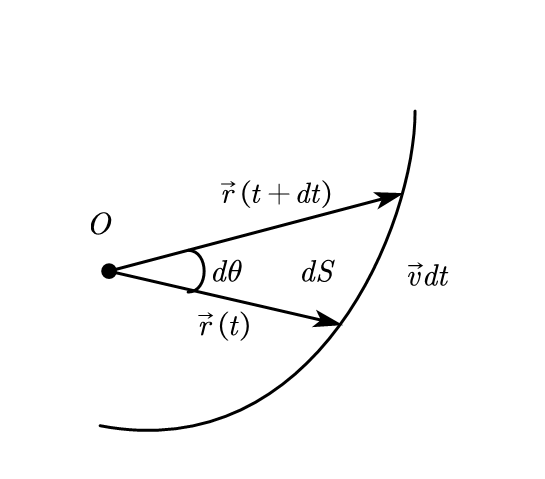
\includegraphics[width = 0.4\textwidth]{figure/掠面速度.png}
        \caption{掠面速度$\kappa$的引入}
        \label{fig:掠面速度}
    \end{figure}

    将这个面积微元矢量化，就得到了我们的掠面速度 $\kappa$
    \begin{equation}
        \vec{\kappa} = \frac{1}{2}\vec{r} \times \vec{v}
    \end{equation}
\end{enumerate}




接下来我们将掠面速度 $\vec{\kappa}$ 与速度 $\vec{v}$ 做一个类比，
\begin{eqnarray*}
    \text{速度} \vec{v} &\Longrightarrow&  \text{动量} \vec{p} = m\vec{v} \\
    \text{掠面速度} \vec{\kappa} &\Longrightarrow&  \text{角动量} \vec{L} = 2m\vec{\kappa}  = \vec{r} \times \vec{p}
\end{eqnarray*}

\begin{remark}
    这里的 $\vec{\kappa},\vec{L}$ 均是相对于不同参考系不同参考点有不同的量，所以无论是学习还是研究，都需要先确定在同一参考系的同一参考点上。
\end{remark}

进一步的，我们有
\begin{eqnarray*}
    \text{速度} \vec{v} &\Longrightarrow&  \text{动量定理} \frac{\mathrm{d\vec{p}}}{\mathrm{d}t} = \vec{F} \\
    \text{掠面速度} \vec{\kappa} &\Longrightarrow&  \text{角动量定理} \frac{\mathrm{d}\vec{L}}{\mathrm{d}t} = \vec{M} 
\end{eqnarray*}

仔细的计算一下我们的角动量 $\vec{L}$ 关于时间的变化规律
\begin{eqnarray*}
     \frac{\mathrm{d}\vec{L}}{\mathrm{d}t}&=& \frac{\mathrm{d} \left(\vec{r} \times \vec{p}\right)}{\mathrm{d}t} \\
     &=& \frac{\mathrm{d}\vec{r}}{\mathrm{d}t} \times \vec{p} + \vec{r} \times \frac{\mathrm{d}\vec{p}}{\mathrm{d}t} \\
     &=& \vec{v} \times \left(m\vec{v}\right) + \vec{r} \times \vec{F} \\
     &=& \vec{r} \times \vec{F}
\end{eqnarray*}

综上，我们得到了角动量定理
\begin{equation}
    \frac{\mathrm{d}\vec{L}}{\mathrm{d}t} = \vec{r} \times \vec{F} = \vec{M}
\end{equation}
在这里，我们给 $\vec{M}$ 一个名字，力矩；而角动量 $\vec{L}$ 也有一个对应的名字，动量矩。

\begin{definition}[角动量（动量矩）]
    质点对某参考点的角动量定义为
    \begin{equation}
        \vec{L} = \vec{r} \times \vec{p} = \vec{r} \times (m\vec{v})
    \end{equation}
    其大小为 $L = mvr\sin\phi$（$\phi$ 为 $\vec{r}$ 与 $\vec{v}$ 的夹角），方向由右手定则确定。
\end{definition}

\begin{definition}[力矩]
    力对某参考点的力矩定义为
    \begin{equation}
        \vec{M} = \vec{r} \times \vec{F}
    \end{equation}
    其大小为 $M = Fr\sin\psi$（$\psi$ 为 $\vec{r}$ 与 $\vec{F}$ 的夹角），方向由右手定则确定。
\end{definition}

\begin{theorem}[角动量守恒定律]
    若质点所受的合力矩为零（$\vec{M} = \vec{0}$），则质点的角动量守恒
    \begin{equation}
        \vec{L} = \vec{r} \times \vec{p} = \text{常矢量}
    \end{equation}
    这等价于：
    \begin{enumerate}
        \item 角动量的大小不变（掠面速度不变）
        \item 角动量的方向不变（运动平面固定）
    \end{enumerate}
\end{theorem}

\begin{remark}
    角动量守恒的条件是"合力矩为零"，而不是"不受力"。万有引力、库仑力等有心力的力矩为零，因此角动量守恒。
\end{remark}

\subsubsection{\protect\hyperlink{:}{角动量的典型例题}}
\addtocontents{toc}{\protect\hypertarget{:}{}}

\begin{example}[角动量守恒——滑冰运动员]
    一个滑冰运动员以角速度 $\omega_1$ 旋转，双臂伸展（转动惯量为 $I_1$）。当她收拢双臂时，转动惯量变为 $I_2$（$I_2 < I_1$）。求新的角速度。
    \begin{solution}
        由角动量守恒（忽略摩擦力矩）
        \begin{equation}
            I_1\omega_1 = I_2\omega_2 \quad \Longrightarrow \quad \omega_2 = \frac{I_1}{I_2}\omega_1
        \end{equation}
        
        由于 $I_2 < I_1$，所以 $\omega_2 > \omega_1$——收拢双臂后转速加快。
    \end{solution}
\end{example}

\begin{example}[角动量守恒——小球在光滑桌面上的运动]
    一个质量为 $m$ 的小球系在轻绳的一端，绳穿过桌面上的小孔，另一端被人拉住。初始时小球在桌面上做半径为 $r_1$ 的圆周运动，速度为 $v_1$。缓慢拉绳使半径变为 $r_2$，求此时的速度。
    \begin{solution}
        绳的拉力始终指向小孔（有心力），力矩为零，角动量守恒
        \begin{equation}
            mr_1 v_1 = mr_2 v_2 \quad \Longrightarrow \quad v_2 = \frac{r_1}{r_2}v_1
        \end{equation}
        
        半径减小，速度增大。动能变化为
        \begin{equation}
            \Delta E_k = \frac{1}{2}mv_2^2 - \frac{1}{2}mv_1^2 = \frac{1}{2}mv_1^2\left(\frac{r_1^2}{r_2^2} - 1\right) > 0
        \end{equation}
        
        动能的增加来自拉绳所做的功。
    \end{solution}
\end{example}

\subsection{\protect\hyperlink{:}{天体运动}}
\addtocontents{toc}{\protect\hypertarget{:}{}}

天体运动是角动量定理和机械能守恒定律的经典应用之一。在这一节中，我们将利用牛顿万有引力定律和角动量守恒来研究天体（如行星绕太阳）的运动轨道。

\subsubsection{\protect\hyperlink{:}{万有引力定律}}
\addtocontents{toc}{\protect\hypertarget{:}{}}

\begin{theorem}[万有引力定律]
    任意两个质点之间存在引力作用，其大小与两个质点质量的乘积成正比，与它们之间距离的平方成反比，方向沿两质点连线方向，即
    \begin{equation}
        \vec{F} = -\frac{GMm}{r^2}\hat{e}_r
    \end{equation}
    其中 $G$ 为万有引力常量，$M$ 和 $m$ 分别为两个质点的质量，$r$ 为两者之间的距离，$\hat{e}_r$ 为从 $M$ 指向 $m$ 的单位矢量。
\end{theorem}

万有引力是一个保守力，其对应的势能为
\begin{equation}
    E_p = -\frac{GMm}{r}
\end{equation}

\subsubsection{\protect\hyperlink{:}{开普勒三定律}}
\addtocontents{toc}{\protect\hypertarget{:}{}}

开普勒在第谷大量天文观测数据的基础上，总结出了行星运动的三条经验定律：

\begin{theorem}[开普勒三定律]
    \begin{enumerate}
        \item \textbf{轨道定律}：所有行星绕太阳运动的轨道都是椭圆，太阳位于椭圆的一个焦点上。
        \item \textbf{面积定律}：从太阳到行星的矢径在相等的时间内扫过相等的面积（即掠面速度守恒）。
        \item \textbf{周期定律}：行星轨道半长轴 $a$ 的立方与公转周期 $T$ 的平方之比为常量，即
        \begin{equation}
            \frac{a^3}{T^2} = \text{常量}
        \end{equation}
    \end{enumerate}
\end{theorem}

值得注意的是，开普勒第二定律（面积定律）实际上就是角动量守恒的直接体现。由于万有引力始终沿径向方向，故力矩 $\vec{M} = \vec{r} \times \vec{F} = \vec{0}$，因此角动量守恒，掠面速度 $\vec{\kappa} = \frac{1}{2}\vec{r} \times \vec{v} = \frac{\vec{L}}{2m}$ 保持不变。

\subsubsection{\protect\hyperlink{:}{轨道方程的推导}}
\addtocontents{toc}{\protect\hypertarget{:}{}}

现在我们来推导在万有引力作用下质点的轨道方程。由于问题具有平面性（角动量守恒保证运动在一个平面内），采用极坐标系 $(r,\theta)$ 是最自然的选择。

由角动量守恒，有
\begin{equation}
    L = mr^2\dot{\theta} = \text{常量}
\end{equation}

利用角动量守恒，我们可以将时间变量替换为角度变量。令 $u = \frac{1}{r}$，则有
\begin{equation}
    \dot{r} = -\frac{1}{u^2}\frac{\mathrm{d}u}{\mathrm{d}\theta}\dot{\theta} = -\frac{L}{m}\frac{\mathrm{d}u}{\mathrm{d}\theta}
\end{equation}

对 $\dot{r}$ 再求一次时间导数
\begin{equation}
    \ddot{r} = -\frac{L}{m}\frac{\mathrm{d}^2 u}{\mathrm{d}\theta^2}\dot{\theta} = -\frac{L^2 u^2}{m^2}\frac{\mathrm{d}^2 u}{\mathrm{d}\theta^2}
\end{equation}

将以上结果代入径向运动方程
\begin{equation}
    m(\ddot{r} - r\dot{\theta}^2) = -\frac{GMm}{r^2}
\end{equation}

化简后得到
\begin{equation}
    \frac{\mathrm{d}^2 u}{\mathrm{d}\theta^2} + u = \frac{GMm^2}{L^2}
\end{equation}

这是一个非齐次线性常微分方程，其通解为
\begin{equation}
    u = \frac{GMm^2}{L^2} + A\cos(\theta - \theta_0)
\end{equation}

其中 $A$ 和 $\theta_0$ 为积分常数。令 $\theta_0 = 0$（选取极轴方向），并定义参数
\begin{equation}
    p = \frac{L^2}{GMm^2}, \qquad e = \frac{AL^2}{GMm^2}
\end{equation}

则轨道方程为
\begin{equation}
    \frac{1}{r} = \frac{1}{p}(1 + e\cos\theta) \quad \Longrightarrow \quad r = \frac{p}{1 + e\cos\theta}
\end{equation}

这正是圆锥曲线的标准方程，其中 $p$ 为半通径，$e$ 为离心率。

\begin{enumerate}
    \item 当 $e = 0$ 时，轨道为圆，$r = p$；
    \item 当 $0 < e < 1$ 时，轨道为椭圆，$p = a(1-e^2)$，$a$ 为半长轴；
    \item 当 $e = 1$ 时，轨道为抛物线；
    \item 当 $e > 1$ 时，轨道为双曲线。
\end{enumerate}

对于椭圆轨道，利用机械能守恒可以证明，轨道总能量为
\begin{equation}
    E = E_k + E_p = -\frac{GMm}{2a}
\end{equation}

这表明：$E < 0$ 对应束缚态（椭圆轨道），$E = 0$ 对应抛物线轨道，$E > 0$ 对应双曲线轨道。

\subsubsection{\protect\hyperlink{:}{宇宙速度}}
\addtocontents{toc}{\protect\hypertarget{:}{}}

利用上述结果，我们可以计算几个重要的宇宙速度：

\begin{enumerate}
    \item \textbf{第一宇宙速度}（环绕速度）：在地表附近作匀速圆周运动所需的最小速度，由 $\displaystyle \frac{mv^2}{R} = \frac{GMm}{R^2}$ 得
    \begin{equation}
        v_1 = \sqrt{\frac{GM}{R}} \approx 7.9 \text{ km/s}
    \end{equation}
    \item \textbf{第二宇宙速度}（逃逸速度）：从地表出发，脱离地球引力束缚所需的最小速度，由能量守恒 $\displaystyle \frac{1}{2}mv_2^2 - \frac{GMm}{R} = 0$ 得
    \begin{equation}
        v_2 = \sqrt{\frac{2GM}{R}} = \sqrt{2}v_1 \approx 11.2 \text{ km/s}
    \end{equation}
    \item \textbf{第三宇宙速度}：从地表出发，脱离太阳系引力束缚所需的最小速度，$v_3 \approx 16.7$ km/s。
\end{enumerate}

\subsubsection{\protect\hyperlink{:}{天体运动的典型例题}}
\addtocontents{toc}{\protect\hypertarget{:}{}}

\begin{example}[椭圆轨道的能量]
    证明椭圆轨道的总能量为 $E = -\frac{GMm}{2a}$，其中 $a$ 为半长轴。
    \begin{solution}
        在近地点（$r_{\min} = a(1-e)$）和远地点（$r_{\max} = a(1+e)$），速度垂直于位矢。由角动量守恒
        \begin{equation}
            mr_{\min}v_{\min} = mr_{\max}v_{\max} = L
        \end{equation}
        
        由机械能守恒
        \begin{equation}
            E = \frac{1}{2}mv_{\min}^2 - \frac{GMm}{r_{\min}} = \frac{1}{2}mv_{\max}^2 - \frac{GMm}{r_{\max}}
        \end{equation}
        
        利用 $r_{\min} + r_{\max} = 2a$ 和 $r_{\min}r_{\max} = a^2(1-e^2) = \frac{L^2}{GMm^2} \cdot a$（由轨道方程），经过计算可得
        \begin{equation}
            E = -\frac{GMm}{2a}
        \end{equation}
    \end{solution}
\end{example}

\begin{example}[卫星轨道变轨]
    一颗卫星在半径为 $r_1$ 的圆轨道上运行。要点火使其进入半径为 $r_2$（$r_2 > r_1$）的圆轨道，求所需的最小速度增量。
    \begin{solution}
        变轨需要经过一个椭圆转移轨道（霍曼转移轨道）。
        
        在 $r_1$ 轨道上的速度：$v_1 = \sqrt{GM/r_1}$
        
        在 $r_2$ 轨道上的速度：$v_2 = \sqrt{GM/r_2}$
        
        转移椭圆的近地点（$r_1$）速度：$v_1' = \sqrt{\frac{GM}{r_1}\cdot\frac{2r_2}{r_1+r_2}}$
        
        转移椭圆的远地点（$r_2$）速度：$v_2' = \sqrt{\frac{GM}{r_2}\cdot\frac{2r_1}{r_1+r_2}}$
        
        第一次点火（在 $r_1$ 处加速）：$\Delta v_1 = v_1' - v_1$
        
        第二次点火（在 $r_2$ 处加速）：$\Delta v_2 = v_2 - v_2'$
        
        总速度增量：$\Delta v = \Delta v_1 + \Delta v_2$
    \end{solution}
\end{example}

\subsubsection{\protect\hyperlink{:}{角动量和天体运动的做题技巧}}
\addtocontents{toc}{\protect\hypertarget{:}{}}

\begin{enumerate}
    \item \textbf{有心力问题用角动量守恒}：当力始终指向某一点（如万有引力、库仑力）时，力矩为零，角动量守恒。
    \item \textbf{轨道问题用极坐标}：天体运动问题中，极坐标系是最自然的选择。利用 $L = mr^2\dot{\theta}$ 可以消去时间变量。
    \item \textbf{能量+角动量双守恒}：天体运动问题中，机械能和角动量都守恒，两个方程联立可以解决大部分问题。
    \item \textbf{圆轨道的特殊性}：圆轨道中，$v = \sqrt{GM/r}$，$E = -GMm/(2r)$，$T = 2\pi r/v = 2\pi\sqrt{r^3/(GM)}$。
    \item \textbf{离心率与能量的关系}：$e = \sqrt{1 + 2EL^2/(G^2M^2m^3)}$，由能量和角动量可以确定轨道形状。
\end{enumerate}


\newpage
\section{\protect\hyperlink{:}{质心、刚体}}
\addtocontents{toc}{\protect\hypertarget{:}{}}

\subsection{\protect\hyperlink{:}{质心、质心运动定理的导出}}
\addtocontents{toc}{\protect\hypertarget{:}{}}

如果说为了给质心找一个比较自然的引入的理由，我想应该是为质点系找一个点位，使得其运动与内力无关，当然，我们一般的教材里面所给出的质心位矢的定义如下：
\begin{definition}
    \begin{equation}
        \vec{r}_c = \dfrac{\sum_i m_i \vec{r}_i}{\sum_i m_i}
    \end{equation}
\end{definition}
可以看出我们的质心是我们的质量分布的一个中心。

既然已经有了质心的位矢，那么也容易得到质心速度为
\begin{equation}
    \vec{v}_c = \frac{\mathrm{d} \vec{r}_c}{\mathrm{d} t} = \frac{\mathrm{d}}{\mathrm{d} t}\left(\frac{\sum_i m_i \vec{r}_i}{\sum_i m_i}\right) = \frac{1}{\sum_i m_i}\frac{\mathrm{d} (\sum_i m_i \vec{r}_i)}{\mathrm{d} t} = \frac{\sum_i m_i \vec{v}_i}{m_c}
\end{equation}

于是我们有
\begin{equation}
    \vec{p}_c = m_c \vec{v}_c = \sum_i m_i \vec{v}_i = \sum_i \vec{p}_i = \vec{p}
\end{equation}

类比于我们的质点的动量定理，我们可以得到
\begin{equation}
    \vec{F}_{\text{合外}} = \frac{\mathrm{d}\vec{p}}{\mathrm{d}t} = \frac{\mathrm{d}\vec{p}_c}{\mathrm{d}t}
\end{equation}

多数情况下，我们的质点系是不会有质量上的变化的，即 $\displaystyle \frac{\mathrm{d} m}{\mathrm{d} t} = 0$，因此，我们有 
\begin{equation}
    \vec{F}_{\text{合外}} = m_c \vec{a}_c
\end{equation}
此即\text{质心运动定理}，这表明，质点系质心的加速度由合外力所确定，与质点系中内力无关，同时我们也获得了一个与牛顿第二定律结构上一致的结论。\\


\begin{example}[质心计算实例]
对于一个线密度为 $\displaystyle \lambda_x = \frac{\lambda_0 x}{L}$ ，长为 $L$ 的一个细杆，求解一下其质心的位置。
    \begin{solution}
        首先给出我们的质量微元 $\displaystyle dm = \lambda_x dx$，以及质心位矢的一个定义式（在这里是一维连续的一个情况），得
        \begin{equation}
            x_c = \frac{\int_{0}^{L} x dm}{\int_{0}^{L} dm} = \frac{\frac{\lambda_0}{L}\int_{0}^{L} x^2 dx}{\frac{\lambda_0}{L}\int_{0}^{L} x dx} = \frac{\frac{1}{3}L^3}{\frac{1}{2}L^2} = \frac{2}{3}L 
        \end{equation}
    \end{solution}

    \begin{remark}
    需要注意的是，在这里我们把求和号直接替换成了积分号，并将一个个离散的质量换成了一系列连续的微元，这在物理的学习当中非常常见.    
    \end{remark}
\end{example}

\subsection{\protect\hyperlink{:}{动力学量在质点系中的分解、质心参考系}}
\addtocontents{toc}{\protect\hypertarget{:}{}}

我们熟知的几个动力学量分别是动量、动能、和角动量，他们也分别对应着力学当中三个重要的守恒方程，是给动力学系统降阶的有力工具，接下来我们将对其进行一个分解
\begin{align*}
    \vec{p} &= \vec{p}_c + \vec{p}^\prime \\
    E_k &= \sum_i \frac{1}{2}m_i v_i^2 \nonumber\\
    &= \sum_i \frac{1}{2} m_i (\vec{v}_c + \vec{v}_i^\prime) \cdot (\vec{v}_c + \vec{v}_i^\prime) \nonumber \\
    &=  \sum_i \frac{1}{2} m_i \left(v_c^2 + 2\vec{v}_c \cdot \vec{v}_i^\prime + v_i^{\prime 2}\right) \nonumber \\
    &= \frac{1}{2} m_c v_c^2 + 2\vec{v}_c \cdot \vec{p}^\prime + \sum_i \frac{1}{2} m_i v_i^\prime \\
    \vec{L} &= \sum_i \vec{r}_i \times (m_i \vec{v}_i) \nonumber \\
    &= \sum_i (\vec{r}_c + \vec{r}_i^\prime) \times m_i(\vec{v}_c + \vec{v}_i^\prime) \nonumber \\
    &= \sum_i m_i(\vec{r}_c \times \vec{v}_c + \vec{r}_c \times \vec{v}_i^\prime + \vec{r}_i^\prime \times \vec{v}_c + \vec{r}_i^\prime \times \vec{v}_i^\prime) \nonumber \\
    &= \vec{L}_c + \vec{r}_c \times \vec{p}^\prime + \sum_i(m_i \vec{r}_i^\prime) \times \vec{v}_c + \sum_i \vec{r}_i^\prime \times (m_i \vec{r}_i^\prime) \nonumber \\
    &= \vec{L}_c + \vec{r}_c \times \vec{p}^\prime + 0 + \vec{L}^\prime \\
    & = \vec{L}_c + \vec{r}_c \times \vec{p}^\prime + \vec{L}^\prime
\end{align*}


而在上一节当中，我们知道，$\displaystyle \vec{p}^\prime = 0$，因此，我们将会得到化简完全的质点系下的动力学量
\begin{align}
    \vec{p} &= \vec{p}_c \\
    E_k &= E_{kc} + 0 + E_k^\prime = E_{kc} + E_k^\prime \\
    \vec{L} &= \vec{L}_c + 0 + \vec{L}^\prime = \vec{L}_c + \vec{L}^\prime
\end{align}

这意味着，对于一个质点系，其动力学量均可以看作是质心的动力学量与质点系中质点相对于质心的动力学量之和，即
\begin{equation*}
    \text{质心的动力学量} + \text{质点系中质点相对于质心的动力学量} = \text{质点系动力学量}
\end{equation*}

这个规律告诉我们，\textbf{当我们在研究质点系的运动时，我们可以将运动的分析放在一个相对于质心不动的参考系中展开，并在最后将其与质心的运动规律相加，即可得到质点系中各个质点的运动状态}，而那个相对于质心不动的参考系称为\textbf{质心参考系}。

\subsection{\protect\hyperlink{:}{刚体}}
\addtocontents{toc}{\protect\hypertarget{:}{}}

刚体的出现是为了解决质点系运动学的"多体困难"，刚体要求质点系中的质点之间的距离是不能够变化的，这使得很多与位置相关的相互作用力不变，这使得我们能够更加轻易的简化问题，但是可能仍然无法解决力的"非线性问题"，但也是走了一大步。

刚体因为其内部的质点都是相互约束的，这就使得我们的刚体在整体上只需要关注一个质点的平动运动就可以确定其他任意一个质点的运动方程，这样平动的自由度直接从 $3n$ 降为了 $3$，同时由于刚体不像质点，它是具有体积的，所以我们除了平动以外，还需要考虑其转动问题，当然，这也是很好解决的，因为 Euler 告诉我们，转动需要三个欧拉角来描述，也就是 $3$ 个自由度，因此，我们的刚体运动的描述一共需要 $6$ 个自由度 
\begin{equation}
    \text{刚体运动的分解}
    \begin{cases}
        \text{随基点的平动} \quad s = 3 \\
        \text{随基点的转动} \quad s = 3
    \end{cases}
\end{equation}


\subsection{\protect\hyperlink{:}{刚体的定轴转动}}
\addtocontents{toc}{\protect\hypertarget{:}{}}
我们之所以研究刚体的定轴转动问题，主要是为了之后研究刚体的平面平行运动，对于平面平行运动，我们如果对刚体的每一个单一质点去描述，将会要求求解非常繁琐的大量变量耦合在一起的微分方程组，因此，我们为了简化刚体运动的描述，我们主要是采取分别研究刚体的定轴转动（将其限制在一个平面内，并且一般是以质心为参考系研究）和刚体的平动问题，这样我们将可以完整的描述整个刚体的运动。

\subsubsection{\protect\hyperlink{:}{刚体定轴转动的运动学量}}
\addtocontents{toc}{\protect\hypertarget{:}{}}

如图 \ref{fig:定轴转动描述} ，我们所描述的是一个质量为 $m$ 的一个刚体，其以 $\vec{\omega}$ 的角速度和 $\vec{\beta}$ 的角加速度绕着一个轴(这里是 $z$ 轴)旋转，为了保证描述的普适性，我们任意取定一个小的质点 $i$ ，其质量为 $m_i$ ，相对于参考点 $O$ 的位矢为 $\vec{r}_i$ ，为了方便描述，我们使用两个分量来描述 $\vec{r}_i = \vec{R}_i + \vec{z}_i$ ，而该质点的线速度为 $\vec{v}_i = \vec{\omega} \times \vec{R}_i$ ，其向心加速度为 $a_{i\text{心}} = \omega^2 R_i$ 切向加速度为 $a_{i\text{切}} = \beta R_i$

\begin{figure}[htbp]
    \centering
    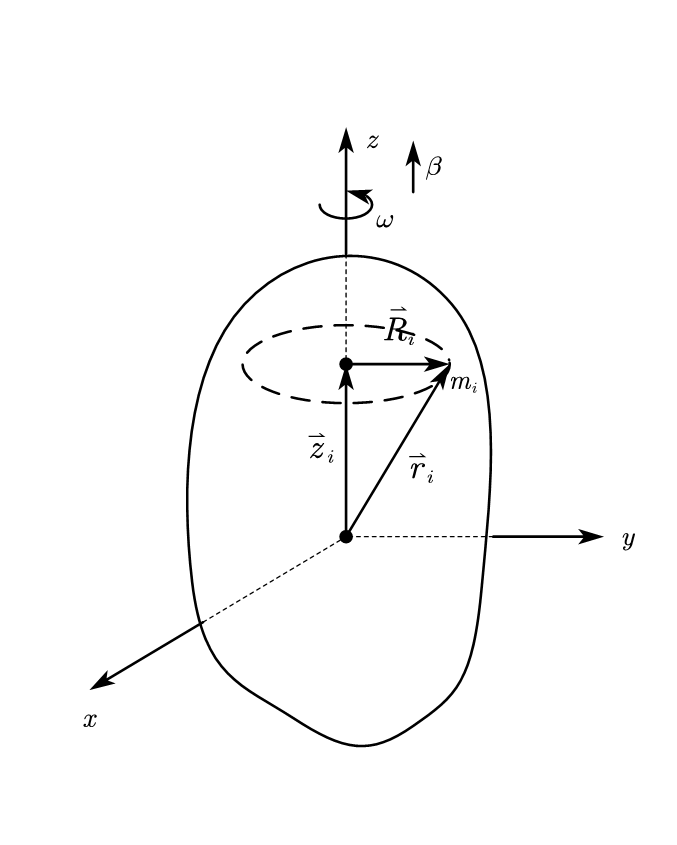
\includegraphics[width=0.4\textwidth]{figure/刚体定轴转动描述.png}
    \caption{刚体定轴转动的描述}
    \label{fig:定轴转动描述}
\end{figure}


\subsubsection{\protect\hyperlink{:}{刚体定轴转动的动力学量}}
\addtocontents{toc}{\protect\hypertarget{:}{}}

基于刚才的一些动力学量的描述，我们将利用他们给出刚体定轴转动的动力学量，比如动量，动能以及角动量，这是我们力学当中求解系统必须的几个物理量。

\paragraph*{动量 $\vec{p}$} 我们知道刚体本身也是一个质点系，因此，其动量 $\vec{p} = \vec{p}_{c}$ ，因此这并没有什么值得讨论的，当我们把系统丢到质心系当中时，系统会立刻变为零动量系。

\paragraph*{动能 $E_k$} 动能的定义也是与质点系是一致的，定义为所有质点的动能之和，即 
\begin{equation*}
    E_k = \sum_i \frac{1}{2}m_i v_i^2 = \sum_i \frac{1}{2}m_i \omega^2 R_i^2 = \frac{1}{2} \left(\sum_i m_i R_i^2\right) \omega^2
\end{equation*}

在这里，我们定义一个新的物理量，转动惯量 $\displaystyle  I = \sum_i m_i R_i^2$ ,这样的话，我们的动能表达式将会变为
\begin{equation}
    E_k = \frac{1}{2} I \omega^2
\end{equation}

这里的转动惯量刚刚好与质点的惯性质量相对应，加速度也刚刚好与质点的速度对应，具有相同的形式。

\paragraph*{角动量 $\vec{L}$} 与上面两个一样，质点系的角动量也是每一个质元的角动量之和，因此写为
\begin{eqnarray*}
    \vec{L} &=& \sum_i \vec{r}_i \times \left(m_i\vec{v}_i\right) \\
    &=& \sum_i m_i \vec{z}_i \times (\vec{\omega} \times \vec{R}_i) + \sum_i m_i \vec{R}_i \times (\vec{\omega} \times \vec{R}_i)
\end{eqnarray*}

在这里，考虑到是绕着 $z$ 轴进行的定轴转动，因此我们仅考虑 $z$ 方向上的角动量，因为只有这个是有影响的，
\begin{eqnarray*}
    L_z &=& \sum_i m_i R_i \omega R_i \\
    &=& \left(\sum_i m_i R_i^2\right) \omega 
\end{eqnarray*}

将其中的 $\displaystyle \sum_i m_i R_i^2$ 替换为转动惯量 $I$ 之后，即为
\begin{eqnarray*}
    L_z = I\omega
\end{eqnarray*}

容易看出，这里的转动惯量刚刚好对应惯性质量，而角速度对应速度，角动量对应动量。


\subsubsection{\protect\hyperlink{:}{刚体的动力学规律}}
\addtocontents{toc}{\protect\hypertarget{:}{}}

有了前面的运动学量和动力学量的定义，我们可以给出刚体定轴转动的动力学规律。

\paragraph*{转动定律} 类比于质点的牛顿第二定律 $\vec{F} = m\vec{a}$，对刚体的定轴转动，我们有

\begin{theorem}[转动定律]
    刚体绕定轴转动时，合外力矩等于转动惯量与角加速度的乘积
    \begin{equation}
        M_z = I\beta = I\ddot{\theta}
    \end{equation}
    其中 $M_z$ 为合外力矩在转轴方向的分量，$I$ 为刚体对转轴的转动惯量，$\beta$ 为角加速度。
\end{theorem}

这一定律可以从角动量定理直接导出：对于定轴转动，$L_z = I\omega$，若 $I$ 不变，则
\begin{equation}
    M_z = \frac{\mathrm{d}L_z}{\mathrm{d}t} = I\frac{\mathrm{d}\omega}{\mathrm{d}t} = I\beta
\end{equation}

\paragraph*{转动惯量的计算} 对于离散质点系，转动惯量的定义为 $I = \sum_i m_i R_i^2$，对于质量连续分布的刚体，则需要将求和替换为积分
\begin{equation}
    I = \int R^2 \mathrm{d}m
\end{equation}

其中 $R$ 是质元 $\mathrm{d}m$ 到转轴的垂直距离。

\begin{theorem}[平行轴定理]
    若已知刚体对通过质心的轴的转动惯量为 $I_c$，则刚体对与该轴平行且相距为 $d$ 的另一轴的转动惯量为
    \begin{equation}
        I = I_c + Md^2
    \end{equation}
    其中 $M$ 为刚体的总质量。
\end{theorem}

一些常见刚体的转动惯量如下：
\begin{enumerate}
    \item 细杆（绕通过中心且垂直于杆的轴）：$\displaystyle I = \frac{1}{12}ML^2$
    \item 细杆（绕通过一端且垂直于杆的轴）：$\displaystyle I = \frac{1}{3}ML^2$
    \item 圆盘/圆柱（绕中心轴）：$\displaystyle I = \frac{1}{2}MR^2$
    \item 球体（绕直径）：$\displaystyle I = \frac{2}{5}MR^2$
    \item 薄球壳（绕直径）：$\displaystyle I = \frac{2}{3}MR^2$
\end{enumerate}

\paragraph*{刚体定轴转动中的功与能} 力矩对刚体做功的定义为
\begin{equation}
    W = \int M_z \mathrm{d}\theta
\end{equation}

类比于质点的动能定理，刚体定轴转动的动能定理为
\begin{equation}
    W = \frac{1}{2}I\omega_B^2 - \frac{1}{2}I\omega_A^2 = \Delta E_k
\end{equation}

其中 $E_k = \frac{1}{2}I\omega^2$ 是刚体绕定轴转动的转动动能。

\paragraph*{刚体定轴转动的角动量守恒} 当合外力矩 $M_z = 0$ 时，角动量守恒
\begin{equation}
    L_z = I\omega = \text{常量}
\end{equation}

如果转动过程中转动惯量发生变化（如人站在转台上收回手臂），则角速度会相应改变以保持角动量守恒，即 $I_1\omega_1 = I_2\omega_2$。


\subsection{\protect\hyperlink{:}{刚体的平面平行运动}}
\addtocontents{toc}{\protect\hypertarget{:}{}}

刚体的平面平行运动是指刚体上任意一点的运动都平行于某一固定平面的运动。例如，一个圆柱在水平面上的纯滚动就是典型的平面平行运动。

对于平面平行运动，我们可以将刚体的运动分解为：
\begin{enumerate}
    \item 随质心的平动：由质心运动定理描述
    \item 绕通过质心且垂直于运动平面的轴的转动：由转动定律描述
\end{enumerate}

\subsubsection{\protect\hyperlink{:}{运动学描述}}
\addtocontents{toc}{\protect\hypertarget{:}{}}

设质心的速度为 $\vec{v}_c$，角速度为 $\vec{\omega}$，则刚体上任意一点 $P$ 的速度为
\begin{equation}
    \vec{v}_P = \vec{v}_c + \vec{\omega} \times \vec{r}_P'
\end{equation}

其中 $\vec{r}_P'$ 是 $P$ 点相对于质心的位矢。

对于圆柱在地面上的纯滚动（无滑动），有一个重要的约束条件：圆柱与地面接触点的瞬时速度为零，即
\begin{equation}
    v_c = R\omega
\end{equation}

其中 $R$ 为圆柱半径。这就是\textbf{纯滚动条件}。

\subsubsection{\protect\hyperlink{:}{动力学方程}}
\addtocontents{toc}{\protect\hypertarget{:}{}}

对于平面平行运动，动力学方程有两个：
\begin{enumerate}
    \item 质心运动定理（平动方程）：
    \begin{equation}
        \vec{F}_{\text{合外}} = M\vec{a}_c
    \end{equation}
    \item 绕质心的转动方程：
    \begin{equation}
        M_c = I_c \beta
    \end{equation}
    其中 $M_c$ 为对质心的合外力矩，$I_c$ 为绕通过质心的转轴的转动惯量。
\end{enumerate}

\subsubsection{\protect\hyperlink{:}{纯滚动圆柱的动力学分析}}
\addtocontents{toc}{\protect\hypertarget{:}{}}

考虑一个质量为 $M$、半径为 $R$ 的圆柱沿倾角为 $\theta$ 的斜面纯滚而下。

设质心加速度为 $a_c$，角加速度为 $\beta$。建立沿斜面向下为正的坐标系。

\paragraph*{平动方程} 沿斜面方向
\begin{equation}
    Mg\sin\theta - f = Ma_c
\end{equation}

其中 $f$ 为静摩擦力（方向沿斜面向上）。

\paragraph*{转动方程} 对质心取矩
\begin{equation}
    fR = I_c\beta
\end{equation}

\paragraph*{纯滚动条件}
\begin{equation}
    a_c = R\beta
\end{equation}

联立以上三个方程，利用 $I_c = \frac{1}{2}MR^2$（实心圆柱），可解得
\begin{equation}
    a_c = \frac{2}{3}g\sin\theta, \qquad f = \frac{1}{3}Mg\sin\theta
\end{equation}

\begin{remark}
    若圆柱作无摩擦的滑动（而非纯滚动），则 $a_c = g\sin\theta$，大于纯滚时的加速度。这说明静摩擦力实际上起到了"让圆柱转动"的作用，使得质心加速度减小，但总动能（平动+转动）仍然符合能量守恒。
\end{remark}

\subsubsection{\protect\hyperlink{:}{纯滚动中的能量}}
\addtocontents{toc}{\protect\hypertarget{:}{}}

纯滚动圆柱的总动能为质心平动动能与绕质心转动动能之和
\begin{equation}
    E_k = \frac{1}{2}Mv_c^2 + \frac{1}{2}I_c\omega^2
\end{equation}

利用纯滚动条件 $v_c = R\omega$，可得
\begin{equation}
    E_k = \frac{1}{2}Mv_c^2 + \frac{1}{2}I_c\frac{v_c^2}{R^2} = \frac{1}{2}\left(M + \frac{I_c}{R^2}\right)v_c^2
\end{equation}

对于实心圆柱（$I_c = \frac{1}{2}MR^2$），有
\begin{equation}
    E_k = \frac{3}{4}Mv_c^2
\end{equation}

利用机械能守恒，可以方便地求解圆柱沿斜面滚下一段距离后质心的速度。


\newpage
\section{\protect\hyperlink{:}{流体力学}}
\addtocontents{toc}{\protect\hypertarget{:}{}}

\begin{definition}[流体]
    流体是指大量的成分相对稳定的物质分子构成的、没有固定形状和具有流动性的物质，一般我们认为流体是液体、气体以及超临界流体，在力学当中只考虑液体和气体。
\end{definition}

考虑到流体虽然相对于刚体而言其内部的作用力要相对较弱，分子间距较大，容易压缩，但是在宏观上也仍然可以处理成连续的质点系，其中的每一个质点都是一个宏观足够小而微观足够大的质元。



\subsection{\protect\hyperlink{:}{流体的静力学}}
\addtocontents{toc}{\protect\hypertarget{:}{}}
与刚体一样，流体中每个质元相互接触的部位也会对彼此施加相互作用力，我们接下来将任意选取一个面元来进行分析。

\begin{figure}[htbp]
    \centering
    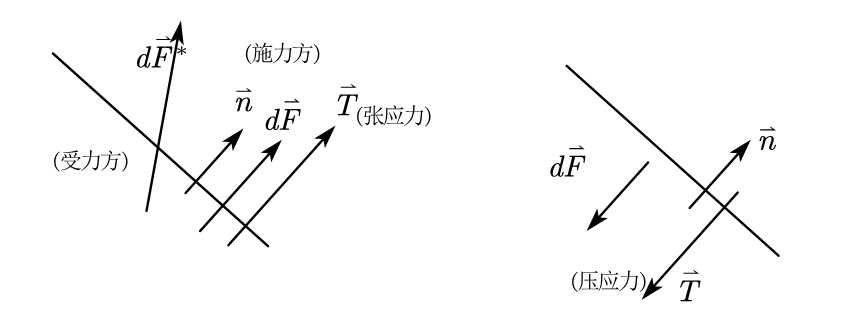
\includegraphics[width=0.8\textwidth]{figure/应力.png}
    \caption{张应力与压应力}
    \label{fig:应力}
\end{figure}

可以看到，若作用力与我们的接触面面元是斜交的一个关系，必然会产生一个切向的分作用，这样的作用将会导致施力方与受力方之间发生相对滑动，如此便与我们所讨论的流体静力学相悖，所以，流体静力学是建立在流体质元之间的相互作用垂直于他们的接触面才能成立的，同时我们还给出了法向应力的概念，这是为了方便静力学的研究，
\begin{definition}
    法向应力被定义为静止流体中真实的作用力 $d \vec{F}$ 与面元的法向量 $\vec{n}$ 相垂直时，作用力与面元面积的比值，即
    \begin{equation}
        \vec{T} = \frac{d \vec{F}}{dS}
    \end{equation}

    另外，我们让 $d\vec{F}$ 与法向量 $\vec{n}$ 同向时称为张应力，反向时称为压应力。
\end{definition}

一般情况下，我们都是考虑压应力，并且利用压应力的概念定义出了压强 $p$ 
\begin{definition}
    压强被定义为压应力的大小，即
    \begin{equation}
        p = \frac{dF}{dS}
    \end{equation}
\end{definition}

另外需要注意的是，对于流体中的任意一个点部分，其压强与其面元的选取是无关的，也即对于各个方向的质元所施加的压应力的大小是一样的。

最后考虑一个简单的情况，重力场下静止流体的压强分布问题，给出示意图
\begin{figure}[htbp]
\centering
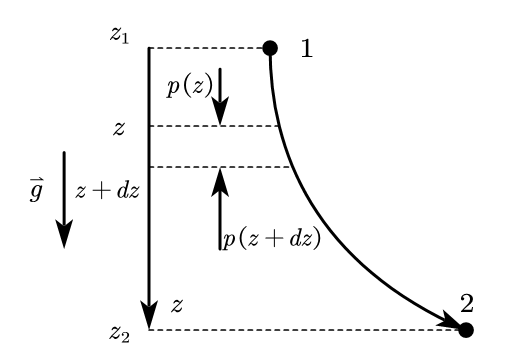
\includegraphics[width=0.5\textwidth]{figure/重力场中压强分布.png}
\caption{重力场中压强分布}
\label{fig:重力场中压强分布}
\end{figure}

从图中，我们可以得到每一个延高度划分的微元所受压强为 $dp = \rho g dz$ ,因此从 $1$ 到 $2$ 的路线过程我们可以得到
\begin{equation}
    \Delta p = p_2 - p_1 = \int_{p_1}^{p_2} = \int_{z_1}^{z_2} \rho g dz = \rho g (z_2 - z_1)
\end{equation}

另外，我们还定义出了一个叫\textbf{浮力} 的概念，
\begin{definition}[浮力]
    外加物体在流体中所受到的来自各个方向上的压力之和未必为 0 ，若有重力的存在，则将会有向上的合压力，称为浮力。
\end{definition}

附加上阿基米德原理，
\begin{theorem}[阿基米德原理]
    浸没在流体中的物体所受到的浮力等于它所排开的流体的重力，即
    \begin{equation}
        \vec{F}_{\text{浮}} = -\rho_{\text{液}} \vec{g} V_{\text{排}}
    \end{equation}
\end{theorem}

\subsection{\protect\hyperlink{:}{流体的运动学}}
\addtocontents{toc}{\protect\hypertarget{:}{}}

关于流体的运动，我们一般在实践中使用两种方法来描述
\begin{enumerate}
    \item 拉格朗日表述：追踪流体中各个质元的位置、速度、加速度随时间的变化
    \item 欧拉表述：关注流体区域内速度的空间分布以及该空间分布随时间的变化
\end{enumerate}

可以看出，拉格朗日表述在使用起来很繁杂，需要很大的算力，因此在日常中，我们主要使用欧拉表述来描述流体的运动。


\subsubsection{\protect\hyperlink{:}{流体的质量守恒及连续性方程}}
\addtocontents{toc}{\protect\hypertarget{:}{}}
现给定一个流体区域 $V$ ，其密度为 $\rho$ ，给出示意图
\begin{figure}[htbp]
\centering
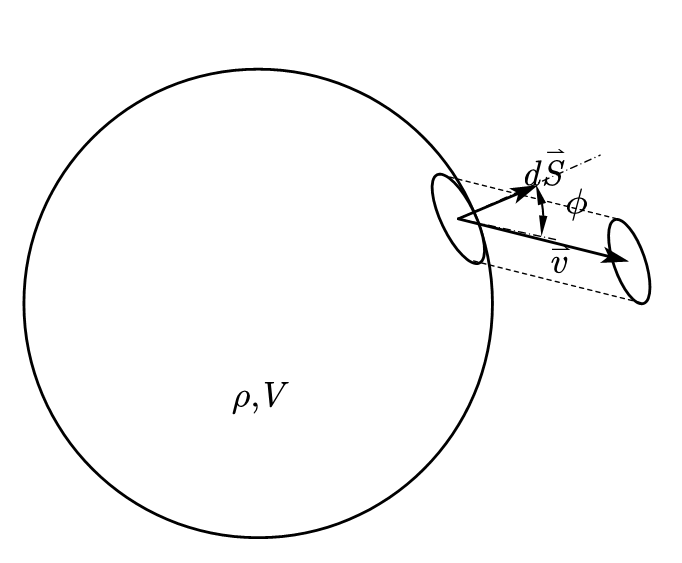
\includegraphics[width=0.4\textwidth]{figure/流体质量守恒.png}
\caption{流体单位时间流出示意图}
\label{fig:质量守恒}
\end{figure}

从图中，我们可以看到，流出流体区域的部分的体积为
\begin{equation*}
    \mathrm{d} V = \mathrm{d} \vec{S} \cdot \vec{v} \mathrm{d} t
\end{equation*}

那么该面元流出去的质量为
\begin{equation*}
    \rho \mathrm{d} V = \rho \mathrm{d} \vec{S} \cdot \vec{v} \mathrm{d} t
\end{equation*}

这只是某个面元所流出的流体，其余的面元也是如此，因此，我们整个面所流出的流体质量为
\begin{equation*}
    \mathrm{d}m = \oiint_S \rho \vec{v} \cdot \mathrm{d} \vec{S} dt
\end{equation*}

接下来，我们可以计算出该流体区域内的质量变化率，首先是给出流体区域内的质量
\begin{equation*}
    m = \iiint_V \rho \mathrm{d}V
\end{equation*}

做一个微元，即可得到流出流体区域的质量变化（注意到这里是减少，应有一个负号）
\begin{equation*}
    -\mathrm{d} m = -\frac{\mathrm{d} m}{\mathrm{d} t} \mathrm{d} t = -\frac{\mathrm{d}}{\mathrm{d} t} \left(\iiint_V \rho \mathrm{d}V\right) \mathrm{d} t
\end{equation*}

考虑到这个流体区域是不随时间变化的，所以有 
\begin{equation*}
    -\mathrm{d} m = -\iiint_V \frac{\partial \rho}{\partial t} \mathrm{d}V \mathrm{d} t
\end{equation*}

另外由于质量守恒，应该有流出量等于质量减少量，则有 
\begin{equation*}
    \oiint_S \rho \vec{v} \cdot \mathrm{d} \vec{S} dt = -\iiint_V \frac{\partial \rho}{\partial t} \mathrm{d}V \mathrm{d} t
\end{equation*}


移个项，除以 $\mathrm{d} t$ ，
\begin{equation}
    \oiint_S \rho \vec{v} \cdot \mathrm{d} \vec{S} + \iiint_V \frac{\partial \rho}{\partial t} \mathrm{d}V = 0
\end{equation}

到了这一步，其实已经是连续性方程了，但我们可以继续利用散度定理（高斯定理）
\begin{equation}
    \oiint_S \vec{A} \cdot \mathrm{d} \vec{S} = \iiint_V \nabla \cdot \vec{A} \mathrm{d}V
\end{equation}

得到
\begin{equation}
    \iiint_V \left(\frac{\partial \rho}{\partial t} + \nabla \cdot (\rho \vec{v})\right) \mathrm{d}V = 0
\end{equation}

此即连续性方程的积分形式。

从这个式子中可以看到，对于那些不可压缩流体（$\rho$ 与空间位置以及时间变化无关）,连续性方程可以被直接化简为 
\begin{equation}
    \oiint_S \vec{v} \cdot \mathrm{d} \vec{S} = 0
\end{equation}


\subsubsection{\protect\hyperlink{:}{流体的定常流动}}
\addtocontents{toc}{\protect\hypertarget{:}{}}

在研究流体的运动时，引入一些几何描述工具是很有帮助的。

\begin{definition}[流线]
    流线是流场中的一条曲线，其上每一点的切线方向都与该点处流体速度 $\vec{v}$ 的方向一致。流线满足微分方程
    \begin{equation}
        \frac{\mathrm{d}x}{v_x} = \frac{\mathrm{d}y}{v_y} = \frac{\mathrm{d}z}{v_z}
    \end{equation}
\end{definition}

\begin{definition}[流管]
    流管是由通过一条封闭曲线上的所有流线所构成的管状曲面。流管内外的流体不会互相穿越。
\end{definition}

\begin{definition}[定常流动]
    若流场中每一点的速度 $\vec{v}$ 仅是空间位置的函数，而不随时间变化，即 $\vec{v} = \vec{v}(\vec{r})$，则称该流动为\textbf{定常流动}（或稳恒流动）。此时流线的形状不随时间变化，流体粒子的运动轨迹（迹线）与流线重合。
\end{definition}

对于定常流动，连续性方程具有特别简洁的形式。考虑一段流管，设截面 $S_1$ 处流速为 $v_1$，密度为 $\rho_1$；截面 $S_2$ 处流速为 $v_2$，密度为 $\rho_2$。由质量守恒，在单位时间内流入 $S_1$ 的质量应等于流出 $S_2$ 的质量
\begin{equation}
    \rho_1 v_1 S_1 = \rho_2 v_2 S_2
\end{equation}

即
\begin{equation}
    \rho v S = \text{常量（沿同一流管）}
\end{equation}

对于不可压缩流体（$\rho = \text{常量}$），上式进一步简化为
\begin{equation}
    v S = \text{常量} \quad \Longrightarrow \quad v_1 S_1 = v_2 S_2
\end{equation}

这表明：在不可压缩流体的定常流动中，流管截面越小的地方，流速越大。

\subsection{\protect\hyperlink{:}{流体动力学}}
\addtocontents{toc}{\protect\hypertarget{:}{}}

\subsubsection{\protect\hyperlink{:}{动量定理}}
\addtocontents{toc}{\protect\hypertarget{:}{}}

对于流体系统，动量定理同样成立。考虑一个流管中的一段流体（称为"流体元"），其两端截面分别为 $S_1$ 和 $S_2$，在 $\mathrm{d}t$ 时间内，这段流体受到的合外力为 $\vec{F}_{\text{合外}}$，其动量的变化率为
\begin{equation}
    \vec{F}_{\text{合外}} = \frac{\mathrm{d}\vec{p}}{\mathrm{d}t}
\end{equation}

在定常流动中，流管内各处的动量分布不随时间变化，因此动量的变化仅来自于流体流入和流出的净效果。对于一段流管中的流体，可以证明
\begin{equation}
    \vec{F}_{\text{合外}} = \oiint_S \rho \vec{v} (\vec{v} \cdot \mathrm{d}\vec{S})
\end{equation}

这是流体动量定理的积分形式，在处理流体对容器壁的作用力等问题中非常有用。

\subsubsection{\protect\hyperlink{:}{能量定理——伯努利方程}}
\addtocontents{toc}{\protect\hypertarget{:}{}}

伯努利方程是流体动力学中最重要的方程之一，它本质上是机械能守恒定律在流体力学中的体现。

考虑不可压缩的理想流体（无粘性）作定常流动。沿一根流管取两个截面 $S_1$ 和 $S_2$，设 $S_1$ 处的压强为 $p_1$、流速为 $v_1$、高度为 $z_1$；$S_2$ 处的压强为 $p_2$、流速为 $v_2$、高度为 $z_2$。

对这段流体应用功能原理，在 $\mathrm{d}t$ 时间内：
\begin{enumerate}
    \item 外力（压力）对流体做功为
    \begin{equation}
        \mathrm{d}W = p_1 S_1 v_1 \mathrm{d}t - p_2 S_2 v_2 \mathrm{d}t
    \end{equation}
    \item 由连续性方程 $S_1 v_1 = S_2 v_2 = Q$（体积流量），设 $\mathrm{d}V = Q\mathrm{d}t$，则
    \begin{equation}
        \mathrm{d}W = (p_1 - p_2)\mathrm{d}V
    \end{equation}
    \item 动能的变化为
    \begin{equation}
        \mathrm{d}E_k = \frac{1}{2}\rho\mathrm{d}V(v_2^2 - v_1^2)
    \end{equation}
    \item 势能的变化为
    \begin{equation}
        \mathrm{d}E_p = \rho g\mathrm{d}V(z_2 - z_1)
    \end{equation}
\end{enumerate}

由功能原理 $\mathrm{d}W = \mathrm{d}E_k + \mathrm{d}E_p$，代入并消去 $\mathrm{d}V$，得到

\begin{theorem}[伯努利方程]
    对于不可压缩理想流体的定常流动，沿同一流管有
    \begin{equation}
        p + \frac{1}{2}\rho v^2 + \rho g z = \text{常量}
    \end{equation}
\end{theorem}

伯努利方程中的三项分别代表：
\begin{enumerate}
    \item $p$：静压强（压强能密度）
    \item $\frac{1}{2}\rho v^2$：动压强（动能密度）
    \item $\rho g z$：重力势能密度
\end{enumerate}

\begin{remark}
    伯努利方程的适用条件为：(1) 不可压缩流体；(2) 理想流体（无粘性）；(3) 定常流动；(4) 沿同一流管。
\end{remark}

伯努利方程有广泛的应用，下面列举几个典型例子：

\paragraph*{小孔流速} 设一个大容器中液面高度为 $H$，容器侧壁底部有一个小孔，液面与小孔处的压强均为大气压 $p_0$。由伯努利方程，取液面和小孔两个截面
\begin{equation}
    p_0 + \frac{1}{2}\rho v_{\text{液面}}^2 + \rho g H = p_0 + \frac{1}{2}\rho v_{\text{孔}}^2 + 0
\end{equation}

由于液面面积远大于小孔面积，$v_{\text{液面}} \approx 0$，因此
\begin{equation}
    v_{\text{孔}} = \sqrt{2gH}
\end{equation}

这就是\textbf{托里拆利公式}，其形式与自由落体的速度公式完全一致。

\paragraph*{文丘里管} 文丘里管是一种测量流速的装置，由一段渐缩管和渐扩管组成。设粗管截面积为 $S_1$，细管截面积为 $S_2$，两处的高度差忽略不计，由伯努利方程和连续性方程联立
\begin{equation}
    p_1 + \frac{1}{2}\rho v_1^2 = p_2 + \frac{1}{2}\rho v_2^2, \qquad v_1 S_1 = v_2 S_2
\end{equation}

可解得
\begin{equation}
    v_1 = S_2\sqrt{\frac{2(p_1 - p_2)}{\rho(S_1^2 - S_2^2)}}
\end{equation}


\newpage
\section{\protect\hyperlink{:}{振动与波}}
\addtocontents{toc}{\protect\hypertarget{:}{}}

振动与波是力学中极为重要的内容，它不仅是经典力学的核心部分，也是理解电磁波、量子力学中波函数等概念的基础。

\subsection{\protect\hyperlink{:}{简谐振动}}
\addtocontents{toc}{\protect\hypertarget{:}{}}

\begin{definition}[简谐振动]
    如果一个质点所受的恢复力与其偏离平衡位置的位移成正比，方向指向平衡位置，即
    \begin{equation}
        F = -kx
    \end{equation}
    则该质点的运动称为\textbf{简谐振动}（SHM），其中 $k > 0$ 为恢复力常量。
\end{definition}

由牛顿第二定律 $F = m\ddot{x}$，得到运动方程
\begin{equation}
    m\ddot{x} = -kx \quad \Longrightarrow \quad \ddot{x} + \omega_0^2 x = 0
\end{equation}

其中 $\omega_0 = \sqrt{k/m}$ 为固有角频率。该方程的通解为
\begin{equation}
    x(t) = A\cos(\omega_0 t + \varphi_0)
\end{equation}

其中 $A$ 为振幅，$\varphi_0$ 为初相位，它们由初始条件 $x(0)$ 和 $\dot{x}(0)$ 确定。

简谐振动的几个重要特征量：
\begin{enumerate}
    \item 周期：$\displaystyle T = \frac{2\pi}{\omega_0}$
    \item 频率：$\displaystyle \nu = \frac{1}{T} = \frac{\omega_0}{2\pi}$
    \item 速度：$\displaystyle v = \dot{x} = -A\omega_0\sin(\omega_0 t + \varphi_0)$
    \item 加速度：$\displaystyle a = \ddot{x} = -A\omega_0^2\cos(\omega_0 t + \varphi_0) = -\omega_0^2 x$
\end{enumerate}

简谐振动的能量为
\begin{equation}
    E_k = \frac{1}{2}m\dot{x}^2 = \frac{1}{2}m\omega_0^2 A^2\sin^2(\omega_0 t + \varphi_0)
\end{equation}
\begin{equation}
    E_p = \frac{1}{2}kx^2 = \frac{1}{2}m\omega_0^2 A^2\cos^2(\omega_0 t + \varphi_0)
\end{equation}

总能量为
\begin{equation}
    E = E_k + E_p = \frac{1}{2}m\omega_0^2 A^2 = \frac{1}{2}kA^2
\end{equation}

总能量守恒，且与振幅的平方成正比。

\subsection{\protect\hyperlink{:}{阻尼振动}}
\addtocontents{toc}{\protect\hypertarget{:}{}}

在实际情况中，振动系统总会受到阻力的作用，导致振幅逐渐减小。最简单的模型是阻力与速度成正比（线性阻尼）
\begin{equation}
    F_{\text{阻}} = -\gamma\dot{x}
\end{equation}

其中 $\gamma > 0$ 为阻尼系数。此时运动方程变为
\begin{equation}
    m\ddot{x} + \gamma\dot{x} + kx = 0 \quad \Longrightarrow \quad \ddot{x} + 2\beta\dot{x} + \omega_0^2 x = 0
\end{equation}

其中 $\beta = \gamma / (2m)$ 为阻尼因子。根据 $\beta$ 与 $\omega_0$ 的大小关系，存在三种情况：

\begin{enumerate}
    \item \textbf{欠阻尼}（$\beta < \omega_0$）：振幅按指数衰减的振荡，解为
    \begin{equation}
        x(t) = A_0 e^{-\beta t}\cos(\omega' t + \varphi_0)
    \end{equation}
    其中 $\omega' = \sqrt{\omega_0^2 - \beta^2}$ 为阻尼振荡角频率。

    \item \textbf{临界阻尼}（$\beta = \omega_0$）：系统最快回到平衡位置而不振荡。

    \item \textbf{过阻尼}（$\beta > \omega_0$）：系统缓慢回到平衡位置，不振荡。
\end{enumerate}

\subsection{\protect\hyperlink{:}{受迫振动与共振}}
\addtocontents{toc}{\protect\hypertarget{:}{}}

当振动系统受到周期性外力的驱动时，会产生\textbf{受迫振动}。设驱动力为 $F_0\cos\omega t$，运动方程为
\begin{equation}
    \ddot{x} + 2\beta\dot{x} + \omega_0^2 x = \frac{F_0}{m}\cos\omega t
\end{equation}

经过足够长的暂态过程后，系统达到稳态，以驱动力的频率作等幅振荡
\begin{equation}
    x(t) = A(\omega)\cos(\omega t - \delta)
\end{equation}

其中稳态振幅为
\begin{equation}
    A(\omega) = \frac{F_0/m}{\sqrt{(\omega_0^2 - \omega^2)^2 + 4\beta^2\omega^2}}
\end{equation}

相位滞后为
\begin{equation}
    \tan\delta = \frac{2\beta\omega}{\omega_0^2 - \omega^2}
\end{equation}

当驱动频率满足 $\omega = \sqrt{\omega_0^2 - 2\beta^2}$ 时，振幅达到最大值，发生\textbf{共振}。当阻尼很小时（$\beta \ll \omega_0$），共振频率近似等于固有频率 $\omega \approx \omega_0$，共振振幅为
\begin{equation}
    A_{\max} \approx \frac{F_0}{2m\beta\omega_0}
\end{equation}

阻尼越小，共振振幅越大。

\subsection{\protect\hyperlink{:}{机械波}}
\addtocontents{toc}{\protect\hypertarget{:}{}}

振动在空间中的传播形成\textbf{波}。机械波的传播需要介质，它本质上是介质中各个质元之间通过弹性力相互耦合而产生的集体振动行为。

\subsubsection{\protect\hyperlink{:}{波动方程}}
\addtocontents{toc}{\protect\hypertarget{:}{}}

一维波动方程描述了波在空间和时间中的传播规律。可以证明，对于一维弹性介质中的小扰动，其位移 $\psi(x,t)$ 满足
\begin{equation}
    \frac{\partial^2 \psi}{\partial x^2} = \frac{1}{v^2}\frac{\partial^2 \psi}{\partial t^2}
\end{equation}

其中 $v$ 为波速。该方程的通解为
\begin{equation}
    \psi(x,t) = f(x - vt) + g(x + vt)
\end{equation}

其中 $f$ 表示沿 $+x$ 方向传播的波，$g$ 表示沿 $-x$ 方向传播的波。

最简单也是最重要的特解是简谐波（正弦波）
\begin{equation}
    \psi(x,t) = A\cos(kx - \omega t + \varphi_0)
\end{equation}

其中 $k = 2\pi/\lambda$ 为波数，$\omega = 2\pi\nu$ 为角频率，$\lambda$ 为波长，$\nu$ 为频率。波速与它们的关系为
\begin{equation}
    v = \frac{\omega}{k} = \lambda\nu
\end{equation}

\subsubsection{\protect\hyperlink{:}{波的能量}}
\addtocontents{toc}{\protect\hypertarget{:}{}}

波在传播过程中携带能量。对于弦上的横波，单位长度的动能和势能相等，总能量密度为
\begin{equation}
    w = \frac{1}{2}\rho\omega^2 A^2
\end{equation}

其中 $\rho$ 为线密度。波的\textbf{强度}（单位时间通过单位截面积的能量）为
\begin{equation}
    I = wv = \frac{1}{2}\rho\omega^2 A^2 v
\end{equation}

波的强度与振幅的平方成正比。

\subsubsection{\protect\hyperlink{:}{波的叠加与干涉}}
\addtocontents{toc}{\protect\hypertarget{:}{}}

\begin{theorem}[叠加原理]
    当两列或多列波同时在同一介质中传播时，介质中每一点的位移等于各列波单独存在时在该点引起的位移的矢量和。
\end{theorem}

当两列频率相同、振动方向相同、相位差恒定的相干波相遇时，会发生\textbf{干涉}现象。设两列波在某点 $P$ 引起的振动分别为
\begin{equation}
    \psi_1 = A_1\cos(\omega t + \varphi_1), \qquad \psi_2 = A_2\cos(\omega t + \varphi_2)
\end{equation}

合成后的振幅为
\begin{equation}
    A^2 = A_1^2 + A_2^2 + 2A_1 A_2\cos\Delta\varphi
\end{equation}

其中 $\Delta\varphi = \varphi_2 - \varphi_1$ 为两列波在该点的相位差。

\begin{enumerate}
    \item 当 $\Delta\varphi = 2n\pi$（$n$ 为整数）时，$A = A_1 + A_2$，干涉相长（加强）
    \item 当 $\Delta\varphi = (2n+1)\pi$ 时，$A = |A_1 - A_2|$，干涉相消（减弱）
\end{enumerate}

若两波源的初相位相同，则相位差仅由波程差 $\delta = r_2 - r_1$ 决定
\begin{equation}
    \Delta\varphi = \frac{2\pi}{\lambda}\delta
\end{equation}

干涉条件简化为：
\begin{enumerate}
    \item 加强：$\delta = n\lambda$（波程差为波长的整数倍）
    \item 减弱：$\delta = (n + \frac{1}{2})\lambda$（波程差为半波长的奇数倍）
\end{enumerate}

\subsubsection{\protect\hyperlink{:}{驻波}}
\addtocontents{toc}{\protect\hypertarget{:}{}}

当两列振幅相同、频率相同、传播方向相反的相干波叠加时，会形成\textbf{驻波}。设两列波为
\begin{equation}
    \psi_1 = A\cos(kx - \omega t), \qquad \psi_2 = A\cos(kx + \omega t)
\end{equation}

叠加后得到
\begin{equation}
    \psi = \psi_1 + \psi_2 = 2A\cos(kx)\cos(\omega t)
\end{equation}

这是一个振幅随位置变化的"驻立"振动：
\begin{enumerate}
    \item \textbf{波腹}：$|\cos(kx)| = 1$，即 $x = n\lambda/2$ 处，振幅最大 $2A$
    \item \textbf{波节}：$\cos(kx) = 0$，即 $x = (n + \frac{1}{2})\lambda/2$ 处，振幅为零
\end{enumerate}

相邻波腹（或波节）之间的距离为 $\lambda/2$，波节与相邻波腹之间的距离为 $\lambda/4$。

驻波中没有能量的定向传播（强度为零的节点除外），能量在波节和波腹之间来回振荡。

\begin{remark}
    弦上的驻波必须满足边界条件。两端固定的弦，两端必须为波节，因此允许的波长为
    \begin{equation}
        \lambda_n = \frac{2L}{n}, \qquad n = 1, 2, 3, \ldots
    \end{equation}
    对应的频率称为\textbf{本征频率}或\textbf{简正频率}：
    \begin{equation}
        \nu_n = \frac{v}{\lambda_n} = \frac{nv}{2L}
    \end{equation}
    其中 $n=1$ 对应\textbf{基频}，$n \geq 2$ 对应\textbf{泛音}（谐波）。
\end{remark}


\newpage
\section{\protect\hyperlink{:}{狭义相对论}}
\addtocontents{toc}{\protect\hypertarget{:}{}}

狭义相对论是爱因斯坦在 1905 年提出的理论，它从根本上改变了我们对时间和空间的认识。

\subsection{\protect\hyperlink{:}{狭义相对论的基本假设}}
\addtocontents{toc}{\protect\hypertarget{:}{}}

\begin{theorem}[狭义相对论的两个基本假设]
    \begin{enumerate}
        \item \textbf{相对性原理}：所有惯性系中，物理定律的形式都是相同的。
        \item \textbf{光速不变原理}：在所有惯性系中，真空中的光速 $c$ 都相同，与光源和观察者的相对运动无关。
    \end{enumerate}
\end{theorem}

\subsection{\protect\hyperlink{:}{洛伦兹变换}}
\addtocontents{toc}{\protect\hypertarget{:}{}}

在伽利略变换下，不同惯性系之间的时间和空间坐标变换为
\begin{equation}
    x' = x - vt, \qquad t' = t
\end{equation}

但伽利兹变换与光速不变原理矛盾。满足相对论两个基本假设的坐标变换为\textbf{洛伦兹变换}。

设惯性系 $S'$ 相对于惯性系 $S$ 以速度 $v$ 沿 $x$ 轴正方向运动，两系的坐标轴平行，且 $t = t' = 0$ 时两原点重合，则洛伦兹变换为
\begin{align}
    x' &= \gamma(x - vt) \\
    y' &= y \\
    z' &= z \\
    t' &= \gamma\left(t - \frac{vx}{c^2}\right)
\end{align}

其中 $\gamma = \dfrac{1}{\sqrt{1 - v^2/c^2}}$ 称为\textbf{洛伦兹因子}。其逆变换为
\begin{align}
    x &= \gamma(x' + vt') \\
    t &= \gamma\left(t' + \frac{vx'}{c^2}\right)
\end{align}

\begin{remark}
    当 $v \ll c$ 时，$\gamma \approx 1$，洛伦兹变换退化为伽利略变换。洛伦兹变换是更一般的变换，伽利略变换只是其低速近似。
\end{remark}

\subsection{\protect\hyperlink{:}{相对论运动学效应}}
\addtocontents{toc}{\protect\hypertarget{:}{}}

\subsubsection{\protect\hyperlink{:}{时间膨胀}}
\addtocontents{toc}{\protect\hypertarget{:}{}}

设在 $S'$ 系中同一地点（$x' = \text{常量}$）发生的两个事件的时间间隔为 $\Delta t' = \tau_0$（称为\textbf{固有时}），则在 $S$ 系中观测到的时间间隔为
\begin{equation}
    \Delta t = \gamma \Delta t' = \gamma \tau_0 = \frac{\tau_0}{\sqrt{1 - v^2/c^2}} > \tau_0
\end{equation}

即运动的时钟走得慢，这就是\textbf{时间膨胀}效应。

\subsubsection{\protect\hyperlink{:}{长度收缩}}
\addtocontents{toc}{\protect\hypertarget{:}{}}

设一根杆在 $S'$ 系中静止，其长度为 $l_0$（称为\textbf{固有长度}），则在 $S$ 系中沿运动方向测量到的长度为
\begin{equation}
    l = \frac{l_0}{\gamma} = l_0\sqrt{1 - v^2/c^2} < l_0
\end{equation}

即运动方向上的长度缩短，这就是\textbf{长度收缩}效应。垂直于运动方向的长度不受影响。

\subsubsection{\protect\hyperlink{:}{速度变换}}
\addtocontents{toc}{\protect\hypertarget{:}{}}

若一个粒子在 $S'$ 系中的速度为 $(u_x', u_y', u_z')$，则在 $S$ 系中观测到的速度为
\begin{align}
    u_x &= \frac{u_x' + v}{1 + \frac{vu_x'}{c^2}} \\
    u_y &= \frac{u_y'}{\gamma\left(1 + \frac{vu_x'}{c^2}\right)} \\
    u_z &= \frac{u_z'}{\gamma\left(1 + \frac{vu_x'}{c^2}\right)}
\end{align}

当 $v, u_x' \ll c$ 时，退化为经典的速度叠加 $u_x = u_x' + v$。特别地，当 $u_x' = c$ 时，$u_x = c$，体现了光速不变性。

\subsection{\protect\hyperlink{:}{相对论动力学}}
\addtocontents{toc}{\protect\hypertarget{:}{}}

为了使牛顿力学与狭义相对论相容，需要对动力学量进行修正。

\subsubsection{\protect\hyperlink{:}{相对论动量与质量}}
\addtocontents{toc}{\protect\hypertarget{:}{}}

相对论中，粒子的动量定义为
\begin{equation}
    \vec{p} = \gamma m_0 \vec{v} = \frac{m_0 \vec{v}}{\sqrt{1 - v^2/c^2}}
\end{equation}

其中 $m_0$ 为粒子的\textbf{静止质量}。有些教材将 $\gamma m_0$ 称为"运动质量" $m = \gamma m_0$，但现代物理学中更倾向于只使用静止质量。

\subsubsection{\protect\hyperlink{:}{相对论能量}}
\addtocontents{toc}{\protect\hypertarget{:}{}}

相对论中，粒子的总能量定义为
\begin{equation}
    E = \gamma m_0 c^2 = \frac{m_0 c^2}{\sqrt{1 - v^2/c^2}}
\end{equation}

当 $v = 0$ 时，得到著名的\textbf{质能关系}
\begin{equation}
    E_0 = m_0 c^2
\end{equation}

总能量与静止能量之差为动能
\begin{equation}
    E_k = E - E_0 = (\gamma - 1)m_0 c^2
\end{equation}

当 $v \ll c$ 时，利用泰勒展开 $\gamma \approx 1 + \frac{v^2}{2c^2}$，可得 $E_k \approx \frac{1}{2}m_0 v^2$，与经典动能一致。

\subsubsection{\protect\hyperlink{:}{能量-动量关系}}
\addtocontents{toc}{\protect\hypertarget{:}{}}

相对论中，能量与动量之间有一个优美的关系。由 $E = \gamma m_0 c^2$ 和 $p = \gamma m_0 v$，可以证明
\begin{equation}
    E^2 = (pc)^2 + (m_0 c^2)^2
\end{equation}

这就是\textbf{能量-动量关系}。对于光子（$m_0 = 0$），有 $E = pc$。

\subsubsection{\protect\hyperlink{:}{相对论力学中的力}}
\addtocontents{toc}{\protect\hypertarget{:}{}}

相对论中，力的定义仍然为动量的变化率
\begin{equation}
    \vec{F} = \frac{\mathrm{d}\vec{p}}{\mathrm{d}t} = \frac{\mathrm{d}}{\mathrm{d}t}(\gamma m_0 \vec{v})
\end{equation}

展开后得到
\begin{equation}
    \vec{F} = \gamma m_0 \vec{a} + \gamma^3 m_0 \frac{\vec{v} \cdot \vec{a}}{c^2}\vec{v}
\end{equation}

可以看到，在相对论中，力与加速度不再同方向（除非力平行或垂直于速度），而且 $\vec{F} = m\vec{a}$ 不再成立。

\begin{remark}
    狭义相对论的核心结论可以概括为：时间和空间不再是独立的绝对量，而是统一的四维时空中的坐标；能量和动量也不再是独立守恒的量，而是统一的四维动量矢量的分量。这一思想深刻影响了现代物理学的发展。
\end{remark}
